
\documentclass[review]{elsarticle}
\usepackage{hyperref}
\usepackage[margin=1in]{geometry}
\usepackage{graphicx}
\usepackage{amsmath}
\usepackage{placeins}
\usepackage{comment}
\usepackage{fancyref}

\def\bibsection{\section*{References}}

\journal{Journal of Nuclear Materials}
\bibliographystyle{elsarticle-num}

\begin{document}
\begin{frontmatter}
\title{A modified Embedded-Atom Method interatomic potential for uranium-silicide}

\author[inl]{Benjamin Beeler\corref{qwe}}
\cortext[qwe]{Corresponding author}
\ead{benjamin.beeler@inl.gov}
\author[lanl,ucsd,msu]{Michael Baskes}
\author[lanl]{David Andersson}
\author[lanl]{Michael Cooper}
\author[inl]{Yongfeng Zhang}
\address[inl]{Idaho National Laboratory, Idaho Falls, ID 83415}
\address[lanl]{Los Alamos National Laboratory, Los Alamos, NM 87545}
\address[ucsd]{University of California-San Diego, San Diego, CA 92093}
\address[msu]{Mississippi State University, MS 39762}


\begin{abstract}

Uranium-silicide (U-Si) fuels are being pursued as a possible accident tolerant fuel (ATF).  This uranium alloy fuel benefits from higher thermal conductivity and higher fissile density compared to uranium dioxide (UO$_{2}$).  In order to perform engineering scale nuclear fuel performance simulations, the material properties of the fuel must be known.  Currently, the experimental data available for U-Si fuels is rather limited.  Thus, multiscale modeling efforts are underway to address this gap in knowledge.  In this study, multiple semi-empirical modified Embedded-Atom Method (MEAM) potentials are presented for the description of the U-Si system.  The potentials are fitted to the formation energy and structural properties of U$_{3}$Si$_{2}$. The primary phase of interest (U$_{3}$Si$_{2}$) is accurately described over a wide temperature range and displays good behavior under irradiation and with free surfaces.  The potentials can also describe a variety of U-Si phases across the composition spectrum.  

\end{abstract}
\end{frontmatter}

\section{Introduction}

Nuclear fuels operate in reactor environments experiencing high temperatures, temperature gradients and mechanical stress under neutron irradiation.  This complex and extreme environment, combined with the high power density that allows nuclear fuels to be economical, presents safety challenges during off-normal events and accidents.  In addition to innovations in reactor design, research is focused on the development of advanced materials \cite{zinkle2016} to improve accident tolerance.  Accident-tolerant fuel (ATF) \cite{zinkle2014} is being considered as a potential fuel type for future and existing light-water reactors (LWRs).  ATFs aim to provide additional coping time in the event of an accident (such as a loss of coolant accident) due to the inherent properties of the fuel, while maintaining good operational characteristics.  Uranium-Silicide (U-Si), and particularly U$_{3}$Si$_{2}$, is being considered as a fuel candidate in ATFs.  U$_{3}$Si$_{2}$ exhibits higher uranium density than traditional UO$_{2}$ LWR fuel, thus allowing for the possibility of reduced enrichments, fewer assemblies and/or an extended lifetime in the core.  U$_{3}$Si$_{2}$ also possesses a higher thermal conductivity than UO$_{2}$, allowing for a lower fuel centerline temperature and more rapid heat removal during off-normal conditions.  

In order for the implementation of U$_{3}$Si$_{2}$ to become a reality, the scientific community must be able to perform continuum scale descriptive and predictive nuclear fuel performance simulations.  To perform such simulations, the material properties of the fuel must be known.  Subjecting U$_{3}$Si$_{2}$ to the in-reactor environment leads to microstructural changes due to the evolution of radiation produced defects, segregation and precipitation of fission products, and mechanical deformation. These changes in fuel microstructure change fuel properties, directly impacting fuel performance and safety.  The ability to understand and model microstructural changes throughout the lifetime of the fuel is critical in developing fuel performance modeling codes.  However, the current experimental data available for U-Si fuels is rather limited.   This includes crystal structures \cite{zachariasen1949, remschnig1992}, phase diagrams \cite{massalski1990}, thermal conductivity, heat capacity, thermal expansion \cite{white2015, shimizu1965}, high pressure diffraction \cite{yagoubi2013}, formation enthalpies \cite{gross1962, ohare1975, alcock1962, rand1963, berche2009} and irradiation studies \cite{shimizu1965, finlay2002}.  Thus, multiscale modeling efforts are underway to address this gap in knowledge.

One recent investigation involved first principles calculations characterizing a variety of properties in the U-Si system \cite{noordhoek2016}.  These calculations have been able to provide insight where experimental information is lacking.  However, first principles calculations are limited in their ability to investigate systems larger than a few hundred atoms in size, and are severely restricted in their ability to investigate properties at non-zero temperatures.  Thus, although these types of investigations are of critical importance, branching to higher time and length scales is necessary for the investigation of larger, more complex systems.  Molecular dynamics-density functional theory (MD-DFT) can be employed to look at non-zero temperatures, but are still restricted to a very small system size and very short time scale.  In order to overcome this limitation, interatomic potentials can be employed within molecular dynamics (MD) methods to solve Newton's equations of motion.  In this way, MD can be used to calculate relevant properties above 0 K on a nanosecond time and nanometer spatial scale.  Information obtained from molecular statics and dynamics simulations can then be input into higher level modeling methodologies such as phase field, kinetic Monte Carlo or continuum level finite element modeling.  In this manner, physics-based multiscale microstructural evolution models can be generated.  Thus, development of an interatomic potential to describe the U-Si system is a critical step in branching time and length scales with the long-term goal of developing a descriptive and predictive nuclear fuel performance code.

Very few interatomic potentials have been constructed for uranium-based alloys.  This is due to the inherent difficulty in describing the behavior of f-electrons and the mechanical instability of the $\gamma$ phase of uranium at low temperatures.   Several interatomic potentials have been developed for pure uranium \cite{beeler_meam, beelerASTM, fernandez2014, li2011, smirnova2012, li2012}, with only a few being adapted into alloy potentials for U-Zr \cite{moore2015},  U-Al \cite{pascuet2012} and U-Mo \cite{smirnovaUMo}.  Based on the functionality of the modified Embedded-Atom Method (MEAM) variants of U and U-Zr \cite{beeler_meam, moore2015} as well as their inclusion of fission gases Xe, Kr and He \cite{beelerASTM}, it is determined that this is a suitable potential form to pursue in attempting to describe the U-Si system.  

This manuscript presents MEAM interatomic potentials for the description of the U-Si system, with particular emphasis on U$_{3}$Si$_{2}$.  No interatomic potentials for the U-Si system have been constructed prior to this work.

 
\section{MEAM Theory}
The Embedded-Atom Method (EAM) \cite{daw1984, daw1993, daw1983} has been shown to predict the properties of alloys and metals quite well. The EAM is the most widely used semi-empirical potential, with applications including calculations of point defects \cite{olsson2009}, melting \cite{belaschenko2011}, grain boundary structure and energy \cite{liu1999}, dislocations \cite{chassange2011} [40], segregation \cite{li2009MatChem}, fracture \cite{vatne2011} and surface structure \cite{rose1984}.  The basis of the EAM is that the cohesive energy can be expressed in terms of embedding energies.  In this view, each atom in the metal is embedded into the electron gas created by the other atoms.  The EAM provides a robust means of calculating structure and energetics; however, it is best suited strictly for purely metallic systems with no directional bonding.
From the EAM, the total energy of a system of atoms is given by equation \ref{eq:eqn1}:


\begin{equation}
\label{eq:eqn1}
E = \sum_{i} \{F(\bar{\rho}_{i})\ +  \frac{1}{2} \sum_{j \neq i} S_{ij}\phi(R_{ij})   \}
\end{equation}

where $i$ and $j$ are the individual atoms of the model \cite{daw1983, daw1984}.  The pair interaction between atoms $i$ and $j$ is given by $\phi$ \cite{baskes1992} and is dependent on the separation between the atoms $R_{ij}$.

\begin{equation}
\label{eq:eqn2}
\phi(R) = \frac{2}{Z} \Bigl\{ E^{u}(R) - F( \frac{ \bar{ \rho}^{0}(R)}{Z}) \Bigr\}  
\end{equation}

In equation \ref{eq:eqn2}, $Z$ is the number of first neighbors, $\bar{ \rho}^{0}(R)$ is the background electron density and $\{E^{u}(R)$ is the per atom energy of the reference structure as a function of nearest-neighbor distance $R$ \cite{baskes2000} obtained from the universal equation of state of Rose et al. \cite{rose1984} given in equation \ref{eq:eqn3}.

\begin{equation}
\label{eq:eqn3}
 E^{u}(R) = -E_{c} (1 + a^{*} + \delta \times (\frac{r_{e}}{r}) \times (a^{*})^{3}) e^{(-a^{*})}
 \end{equation}

with

\begin{equation}
\label{eq:eqn4}
a^{*} = \alpha ( \frac{R}{r_{e}} - 1)
\end{equation}

and

\begin{equation}
\label{eq:eqn5}
\alpha^{2} = \frac{9\omega B}{E_{c}}
\end{equation}

where E$_{c}$, r$_{e}$, $\omega$ and B are the cohesive energy, nearest neighbor distance, atomic volume and bulk modulus, respectively, evaluated at equilibrium in the reference structure.  The background electron density is given by:

\begin{equation}
\label{eq:eqn6}
\bar{\rho}^{0}(R) = Z \rho^{a(0)} (R)
\end{equation}

where $\rho^{a(0)}$  is an atomic electron density discussed below.  The embedding function, F, is given in equation \ref{eq:eqn7} and is the energy required to embed atom i into a system with a background electron density $\bar{\rho}_{i}$.  

\begin{equation}
\label{eq:eqn7}
F(\bar{\rho}) = AE_{c} \frac{\bar{\rho}}{Z}\ln\frac{\bar{\rho}}{Z}
\end{equation}

The modification to the EAM is a function of how the electron density at a certain point, $\rho_{i}$, is calculated.  In the traditional EAM, $\rho_{i}$ is simply the linear supposition of spherically averaged atomic electron densities:

\begin{equation}
\label{eq:eqn8}
\rho_{i}^{(0)} = \sum_{j \neq i} \rho_{j}^{a(0)} (R_{ij})
\end{equation}

whereas the MEAM introduces angularly dependent terms to augment $\bar{\rho_{i}}$ as shown in equation \ref{eq:eqn9} through equation \ref{eq:eqn11} \cite{baskes2000, baskes1987}.  

\begin{equation}
\label{eq:eqn9}
(\rho_{i}^{(1)})^{2}=\sum_{\alpha} \{ \sum_{j \neq i}x_{ij}^{\alpha}\rho_{i}^{a(1)}(R_{ij})\}^{2} = \sum_{j,k \neq i}\rho_{j}^{a(1)}(R_{ij})\rho_{k}^{a(1)}(R_{ik})cos\{\theta_{ijk}\}
\end{equation}

\begin{equation}
\label{eq:eqn10}
(\rho_{i}^{(2)})^{2}=\sum_{\alpha,\beta}\{\sum_{j \neq i}x_{ij}^{\alpha}x_{ij}^{\beta}\rho_{j}^{a(2)}(R_{ij})\}^{2} - \frac{1}{3}\sum_{j \neq i}[\rho_{j}^{a(2)}(R_{ij})]^2
\end{equation}

\begin{equation}
\label{eq:eqn11}
(\rho_{i}^{(3)})^{2}=\sum_{\alpha,\beta,\gamma}\{ \sum_{j \neq i}x_{ij}^{\alpha}x_{ij}^{\beta}x_{ij}^{\gamma}\rho_{j}^{a(3)}(R_{ij}) \}^{2} - \frac{3}{5}\sum_{j \neq i}[\rho_{j}^{a(3)}(R_{ij})]^2
\end{equation}

Here, the $\rho^{a(l)}$  are the atomic densities which represent the decrease in the contribution with distance R$_{ij}$ and the $\alpha$, $\beta$, $\gamma$ summations are each over the three coordinate directions with x$_{ij}^{\alpha}$ being the distance the ratio R$_{ij}^{\alpha}$/R$_{ij}$ with R$_{ij}^{\alpha}$ being the $\alpha$ component of the distance vector between atoms i and j [29].  Similar to equation \ref{eq:eqn9}, equations \ref{eq:eqn10} and \ref{eq:eqn11} can be put in a form that has a dependence on the angle between atoms i, j and k ($\theta_{ijk}$), and this has been done by Baskes et al. \cite{baskes1989}.  Atomic electron densities are assumed to decrease exponentially, 

\begin{equation}
\label{eq:eqn12}
\rho_{i}^{a(l)}(R) = e^{[-\beta^{(l)}(\frac{R}{r_{e}}-1)]}
\end{equation}

where $\beta^{(l)}$ are the decay lengths.  To obtain the background electron density from the partial electron densities we make the assumption that the angular terms are a small correction to the EAM.

\begin{equation}
\label{eq:eqn13}
(\rho_{i}^{(0)})^{2} = \sum_{l=0}^{3}\bar{t}_{i}^{(l)} (\rho_{i}^{(l)})^{2}
\end{equation}

where the $\bar{t}_{i}^{(l)}$ \cite{valone2006} are combinations of model constants $t^{l}$ that are associated with the atom types of neighbors $i$.

Many body screening is implemented through a screening function, S$_{ij}$, that quantifies screening between two atoms i and j due to other atoms in the system, k.  The atomic electron densities and the pair potential are multiplied by this function.  The screening function depends on all other atoms in the system:

\begin{equation}
\label{eq:eqn14}
S_{ij}=\Pi_{k \neq i,j}S_{ijk}
\end{equation}

where S$_{ijk}$ is calculated using a simple geometric construction.  The screening factor S$_{ijk}$ is defined as:

\begin{equation}
\label{eq:eqn15}
S_{ijk}= f_{c}\left[\frac{C-C_{min}}{C_{max}-C_{min}}\right]
\end{equation}

where C is a geometric parameter, and C$_{min}$ and C$_{max}$ are limiting values of C.  The smooth cutoff function is:

\begin{equation}
\label{eq:eqn16}
f_{c}(x) = \begin{cases}
    1       & \quad x \geq 1 \\
    [1-(1-x)^{6}]^{2}  & \quad 0 < x < 1\\
    0       & \quad x \leq 0\\
  \end{cases} 
\end{equation}

A radial cutoff function is also applied to the atomic electron densities and pair potential which is given by f$_{c}[(r_{c}-r)/\lambda]$ where r$_{c}$ is the cutoff distance of 6 {\AA } and $\lambda$ gives the cutoff region and was chosen to be 0.1.  The MEAM has been shown to accurately predict the behavior of complex systems such as plutonium \cite{baskes2000} and tin \cite{baskes1997}.  It should be noted that these equations are for a single component system and can be generalized for a multicomponent system, as was done in \cite{baskes2014}.  

\section{Fitting Procedure}
In order to create a functional uranium-silicide (U-Si) binary interatomic potential, there must first exist (or be generated) suitable potentials for each individual element.  A uranium potential from Moore, $\textit{et al.}$ \cite{moore2015} is utilized in the fitting.  This MEAM interatomic potential performs excellently in describing the body-centered cubic phase of uranium and the alloy behavior of UZr.  For the Si MEAM contribution, the initial potential utilized was from Baskes \cite{baskes1992}.  Upon finding this potential over-predicted the Si-Si dimer distance (compared to the reference value of 2.25 \AA \cite{huber1979}), the fitting of a new Si-Si potential was undertaken in an attempt to rectify this discrepancy, as well as increasing the vacancy formation energy in diamond cubic silicon.  Initially, an updated silicon potential was generated by only allowing a restricted set of MEAM parameters to vary: $\beta$$^{0}$, $\beta$$^{1}$, $\beta$$^{2}$, $\beta$$^{3}$, $t$$^{1}$, C$_{min}$ and C$_{max}$.  The resulting potential is shown in Table \ref{tab:ben1}, denoted as Si-MEAM A, with the associated 0 K properties of the original and new MEAM potentials shown in Table \ref{tab:ben2}.  Although the Si-Si dimer distance was unchanged, the formation energy of a vacancy in diamond Si is increased.  All other 0 K properties are relatively unaffected.  This potential was deemed suitable to proceed.  One drawback of this newer Si potential is a lower predicted melting point than the experimental value.  Thus, a secondary fitting was undertaken that allowed all MEAM parameters to change, except for the information regarding the reference structure, with the goal of increasing the melting point.  The resulting potential is shown in Table \ref{tab:ben1}, denoted as Si-MEAM B, with the associated 0 K properties shown in Table \ref{tab:ben2}.  Finally, it was observed that both of these Si MEAM potentials greatly overestimated the thermal expansion of diamond cubic silicon, and thus a third fitting procedure was undertaken with an emphasis on more accurately predicting the thermal expansion.  This third MEAM potential is shown in Table \ref{tab:ben1} and denoted as Si-MEAM C, with the associated 0 K properties shown in Table \ref{tab:ben2}.   All three Si potentials were pursued for the development of a U-Si MEAM binary potential.  

\begin{table}[h]
\caption{Silicon MEAM potential parameters}\label{tab:ben1}
\begin{center}
\begin{tabular}{|c|c|c|c|c|}
     \hline
     Parameter & Original Si-MEAM  & Si-MEAM A & Si-MEAM B  & Si-MEAM C \\
     \hline
     attrac & 0 & 0 & -0.1817 & -0.1597 \\
     repuls & 0 & 0 & 0.107 & -0.1978 \\
     alpha & 4.87 & 4.87 & 5.0411 & 5.4907 \\
     $\beta$$^{0}$ & 4.4 & 4.4662 & 5.5805 & 4.1478 \\
     $\beta$$^{1}$ & 5.5 & 9.4016  & 10.0569 & 5.678\\
     $\beta$$^{2}$ & 5.5 & 13.3826 & 12.9925 & 4.5213 \\  
     $\beta$$^{3}$ & 5.5 & 8.6993 & 9.7566 & 5.4731 \\
     alat (\AA) & 5.431 & 5.431 & 5.431 & 5.431 \\
     E$_{c}$ (eV) & 4.63 & 4.63 & 4.63 & 4.63\\
     A & 1 & 1 & 1.278 & 0.7929\\
     t$^{0}$ & 1 & 1 & 1 & 1\\
     t$^{1}$ & 2.05 & 2.8841 & 1.9557 & 2.028 \\
     t$^{2}$ & 4.47 & 4.47 & 4.411 & 4.6003\\
     t$^{3}$ & -1.80 & -1.80  & -1.7684 & -1.2871\\
     C$_{min}$ & 2.0 & 1.7215 & 1.6299 & 0.8784 \\ 
     C$_{max}$ & 2.8 & 2.4942 & 2.6209 & 2.7211 \\
     \hline
\end{tabular}
\end{center}
\label{default}
\end{table}%

\begin{table}[h]
\caption{Properties of silicon MEAM potentials.  Units are as follows: E (eV/atom), a (\AA), c$_{xx}$ (GPa), E$_{form}$ (eV).     }\label{tab:ben2}
\begin{center}
\begin{tabular}{|c|c|c|c|c|c|}
     \hline
     Structure & Property & Original Si-MEAM  & Si-MEAM A & Si-MEAM B & Si-MEAM C\\
     \hline
     Diamond & E & -4.63 & -4.63 & -4.63 & -4.63\\
     & a & 5.431 & 5.431 & 5.431 & 5.431\\
     & c$_{11}$ & 163.8 & 165.2 & 188.5 & 183.3\\
    & c$_{12}$  & 64.6 &	64.6  & 63.3 & 94.4\\
 & c$_{44}$ & 78.8	& 95.2 & 101.6 & 67.2\\
& E$_{form}^{vac}$ &3.858 & 4.142 & 4.996 & 3.553\\
    \hline
FCC & E &-4.065 &	-4.151 & -3.061 & -3.978\\
& a & 4.100 &	4.098 & 4.046 & 3.777\\
    \hline
HCP &  E &-4.067 &	-4.152 & -3.063 & -3.988 \\
& a & 2.904 &	2.902 & 2.863 & 2.672\\
& c/a & 1.624 &	1.624 & 1.628 & 1.628\\ 
    \hline
SC & E & -4.337 &	-4.358 & -4.011 & -4.462\\
& a &2.622 &	2.622 & 2.626 & 2.516\\
    \hline
BCC & E & -4.316 &	-4.286 & -3.085 & -3.232\\
& a & 3.145 &	3.176 & 3.195 & 3.009\\
    \hline
Dimer & E & -2.558 &	-2.546 & -2.941 & -2.208\\
& a & 2.431 &	2.443 & 2.420 & 2.428\\
           \hline
\end{tabular}
\end{center}
\label{default}
\end{table}%

The fitting procedure to develop cross-species parameters (U-Si interactions) involves a reference phase (L1$_{2}$-U$_{3}$Si), a starting guess for MEAM parameters, and is then refined via a script that gives a random step to all relevant MEAM parameters.  This updated potential is then input into LAMMPS \cite{plimpton1995} and a series of simulations are performed, the output of which is utilized to calculate a weighted-error summation.  The script then either accepts or rejects the prescribed changes to the MEAM parameters based on the reduction of the total weighted-error.  The emphasis of the fitting procedure was the U$_{3}$Si$_{2}$ phase, which possesses a relatively complex crystal structure, with a 10 atom unit cell in space group P4/$\textit{mbm}$-No. 127, two unique uranium atomic sites (2a (0, 0, 0) and 4h (0.181, 0.681, 0.5) ) and one unique silicon atomic site (4g (0.389, 0.889, 0) ), as first reported by Zachariasen \cite{zachariasen1949}.  The cohesive energy, lattice constants and elastic constants of the U$_{3}$Si$_{2}$ phase were given priority with respect to the error weighting, and are thus considered the primary fitting targets.  Additionally, a number of alternative structures were discovered throughout the fitting procedure via a heating and quenching simulation.  Up to eight alternative structures were included as fitting targets at a given time, enforcing the condition that these structures exhibited a higher energy than the experimental structure.  The Si vacancy formation energy was only included into the fitting of the U-Si MEAM B potential.  A variety of other simulations were performed periodically to serve as sanity checks for the potential, the entirety of which is beyond the scope of this paper.  The potential parameters are shown in Table \ref{tab:ben3}, with the U-Si MEAM A potential utilizing the Si-MEAM A potential, the U-Si MEAM B potential utilizing the Si-MEAM B potential and the U-Si MEAM C potential utilizing the Si-MEAM C potential.  Screening parameters are given in LAMMPS format (i.e., C$_{max}$(I,J,K) is a screening parameter when I-J pair is screened by K, where I, J and K are atom types).  



\begin{table}[h]
\caption{Uranium-silicon MEAM potential parameters.  Uranium is atom type 1 and silicon is atom type 2.}\label{tab:ben3}
\begin{center}
\begin{tabular}{|c|c|c|c|}
     \hline
     Parameter & U-Si MEAM A & U-Si MEAM B & U-Si MEAM C \\
     \hline
     E$_{c}$ (eV) & 5.36 & 5.36 & 5.36\\ 
     r$_{e}$ (\AA) & 3.05 & 3.05 & 3.05\\
     lattce & l12 & l12 & l12\\
     r$_{c}$ (\AA) & 6.0 & 6.0 & 6.0\\
     attrac & 0.1873 & 0.1627 & -0.1932 \\
     repuls & 0.0742 & 0.1156 & 0.1663 \\
     alpha(1,2) & 4.978 & 5.061 &4.6574 \\
     rho(2) & 4.151 & 4.191 & 1.0992\\
     rho(1) & 1 & 1 & 1\\
     C$_{min}$(1,1,2) & 0.124 & 0.145 & 0.893\\
     C$_{max}$(1,1,2) & 2.604 & 2.737 & 2.337\\
     C$_{min}$(1,2,1) & 2.107 & 2.494 & 0.195\\
     C$_{max}$(1,2,1) & 2.741 & 2.727 & 1.851\\
     C$_{min}$(1,2,2) & 1.549 & 1.598 & 0.977\\
     C$_{max}$(1,2,2) & 2.517 & 2.461 & 2.765\\
     C$_{min}$(2,2,1) & 0.985 & 0.989 & 1.121\\  
     C$_{max}$(2,2,1) & 1.606 & 1.63 & 1.397\\
     \hline
\end{tabular}
\end{center}
\label{default}
\end{table}%

For the sake of clarity and reproducibility, LAMMPS MEAM-specific parameters are included in Table \ref{tab:ben4}.  It should also be noted that a non-standard implementation of MEAM within LAMMPS (which relates to modification of the smooth cutoff function) was utilized for the existing U MEAM potential and the subsequent U-Si potentials.  Please contact the authors to obtain the required modifications in order to accurately utilize the potential.  

\begin{table}[h!]
\caption{LAMMPS MEAM-specific parameters \cite{plimpton1995}.}\label{tab:ben4}
\begin{center}
\begin{tabular}{|c|c|}
     \hline
     Parameter & U-Si MEAM  \\
     \hline
     bkgd\_dyn & 1 \\
     nn2 & 1 \\
     delr (\AA)& 0.1 \\
     ialloy & 1 \\
     augt1 & 0 \\
     emb\_lin\_neg & 1 \\
     \hline
\end{tabular}
\end{center}
\label{default}
\end{table}%

\clearpage

\section{U-Si MEAM Potential Results}

The results for fundamental properties of U$_{3}$Si$_{2}$ at 0 K are displayed in Table \ref{tab:ben5} and compared to experiments \cite{zachariasen1949, berche2009} and DFT calculations \cite{noordhoek2016} (DFT+U results from \cite{noordhoek2016} are used for comparison but are simply referred to as DFT here).  For the U-Si MEAM A potential, the formation energy and the volume per atom are very accurate.  The $\it{a}$ lattice constant is slightly underestimated and the $\it{c}$ lattice constant is slightly overestimated.  The elastic constants show varying degrees of agreement with DFT predictions.  Excellent agreement shown for G$^{xy}$ and G$^{xz}$ (equations \ref{eq:gxy} and \ref{eq:gxz}), but significant variance is observed for C$_{44}$, for example.  The resulting bulk modulus, calculated via the elastic constants in equation \ref{eq:bulk}, is overestimated.  The bulk modulus was also calculated via the Birch-Murnaghan curve \cite{cohen85, birch47}, yielding a value of 114 GPa, which is consistent with the calculation of the bulk modulus via elastic constants.  There is observed a general over-stiffness prediction of the elastic constants, with the exception being C$_{44}$, which is under-predicted.  The root-mean-square error over the nine calculated elastic constants is 38.8 GPa.  

For the U-Si MEAM B potential an over-prediction of the formation energy of 0.1 eV/at is observed.  The predicted volume per atom is quite accurate, with the same under-prediction of the $\it{a}$ lattice constant and over-prediction of the $\it{c}$ lattice constant as in U-Si MEAM A.  The elastic constants are generally over-stiff, particularly in the case of C$_{11}$ and C$_{66}$.  The resulting bulk modulus and shear elastic constants are also over-stiff by a larger degree than that for U-Si MEAM A.  The root-mean-square error over the nine calculated elastic constants is 84.5 GPa.

The U-Si MEAM C potential accurately predicts the formation energy per volume, as well as the $\it{c}$ lattice constant, while underestimating the $\it{a}$ lattice constant and the volume per atom.  This results in a more accurate prediction of the $\it{c/a}$ ratio than the other two potentials.  The elastic constants generally show an over-stiff prediction when compared to experiment, with the exceptions of C$_{33}$ and C$_{66}$.  The root-mean-square error over the nine calculated elastic constants is 55.9 GPa.  

\begin{equation}
\label{eq:gxy}
G^{xy}= \frac{\frac{C_{11} + C_{22}}{2} - C_{12}}{2}
\end{equation}

\begin{equation}
\label{eq:gxz}
G^{xz}= \frac{\frac{C_{11} + C_{33}}{2} - C_{13}}{2}
\end{equation}

\begin{equation}
\label{eq:bulk}
B=(C_{11} + C_{22} + C_{33} + 2*C_{12} + 2*C_{13} + 2*C_{23})/9
\end{equation}

\begin{table}[h!]
\caption{Properties of U$_{3}$Si$_{2}$ at 0 K.  Results from the MEAM U-Si potential are compared to experiments$^{1}$\cite{zachariasen1949}$^{2}$\cite{berche2009} and DFT$^{3}$\cite{noordhoek2016} calculations.  Units are as follows: E (eV/atom), V/at (\AA$^{3}$/atom), a and c (\AA), C$_{xx}$, B and G (GPa). }\label{tab:ben5}
\begin{center}
\begin{tabular}{|c|c|c|c|c|}
     \hline
      & Reference & U-Si MEAM A & U-Si MEAM B & U-Si MEAM C \\
     \hline
     E & -0.356$^{2}$ & -0.354 & -0.259 & -0.335\\
     V/at & 20.844$^{1}$ & 20.950 & 21.004 & 19.660\\
     a & 7.32$^{1}$ & 7.157 & 7.177 & 7.077\\
     c & 3.89$^{1}$ & 4.090 & 4.078 & 3.925\\
     c/a & 0.531$^{1}$ & 0.572 & 0.568 & 0.555\\
     C$_{11}$ & 149$^{3}$ & 196.6 & 270.4 & 163.8 \\
     C$_{33}$ & 139$^{3}$ & 152.3 & 182.6 & 93.0\\
     C$_{12}$ & 49$^{3}$ & 81.9 & 49.7 & 137.4\\
     C$_{13}$ & 48$^{3}$ & 77.0 & 92.8 & 83.6\\
     C$_{44}$ & 63$^{3}$ & 15.3 & 12.1 & 177.6\\
     C$_{66}$ & 46$^{3}$ & 105.8 & 236.8 & 26.5\\
     B & 81$^{3}$ & 113 & 133 & 114\\
     G$^{xy}$ & 50$^{3}$ & 57 & 110 & 13  \\
     G$^{xz}$ & 48$^{3}$ & 49 & 67 & 22\\
     \hline
\end{tabular}
\end{center}
\label{default}
\end{table}%

The U$_{3}$Si$_{2}$ structure is shown in Figure \ref{fig:ben1} \cite{zachariasen1949}.  This figure illustrates a supercell of 2$\times$2$\times$3 unit cells with periodic boundaries.  In comparing the experimental structure to the predicted structures from the MEAM potentials, all potentials exhibit similar minute differences.  There exists a slight expansion of uranium atoms (red) in the purely uranium plane and a minuscule clockwise rotation of atoms in the unit cell, with respect to the experimental structure.  This alteration is nearly imperceptible, except by analyzing the radial distribution functions (RDFs), as shown in Figure \ref{fig:benrdf}.  The RDF shows that the predicted structure from the MEAM potentials is not capturing the smallest interatomic distance; this is due to the slight expansion in the U plane and the clockwise rotation of U and Si atoms.  These minor distortions slightly increase the first nearest neighbor distance by approximately 0.2 {\AA} and slightly decrease the second and third nearest neighbor distances, as shown in Figure \ref{fig:benrdf} in the distance regime of 2.8-3 {\AA}.  The first nearest-neighbor distance is a Si-Si distance.  It is possible this is overestimated due to the inherent properties of the Si MEAM potentials, which over-predicts the Si-Si dimer distance.  

\begin{figure}[ht]
	\centering
	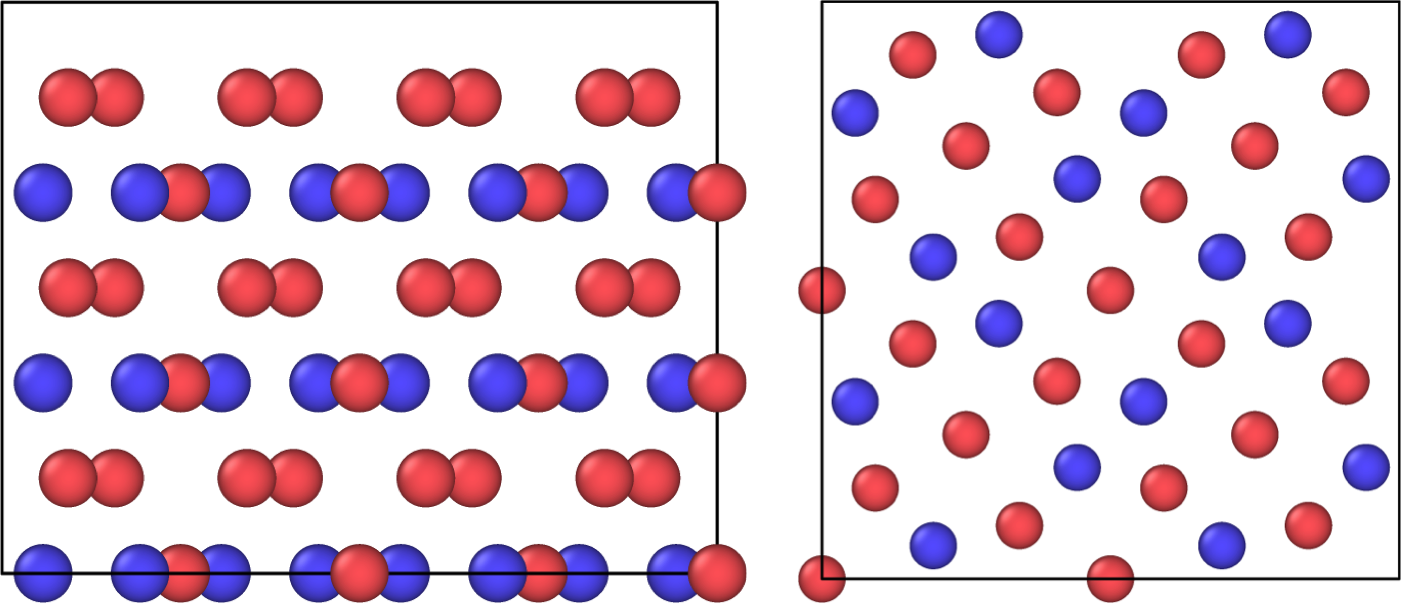
\includegraphics[width=0.8\textwidth]{ben1NEW.png}
    \caption{(100) view (left) and (001) view (right) of the experimental structure of U$_{3}$Si$_{2}$.  Uranium atoms in red; Silicon atoms in blue.}\label{fig:ben1}
\end{figure}  

\begin{figure}[ht]
	\centering
	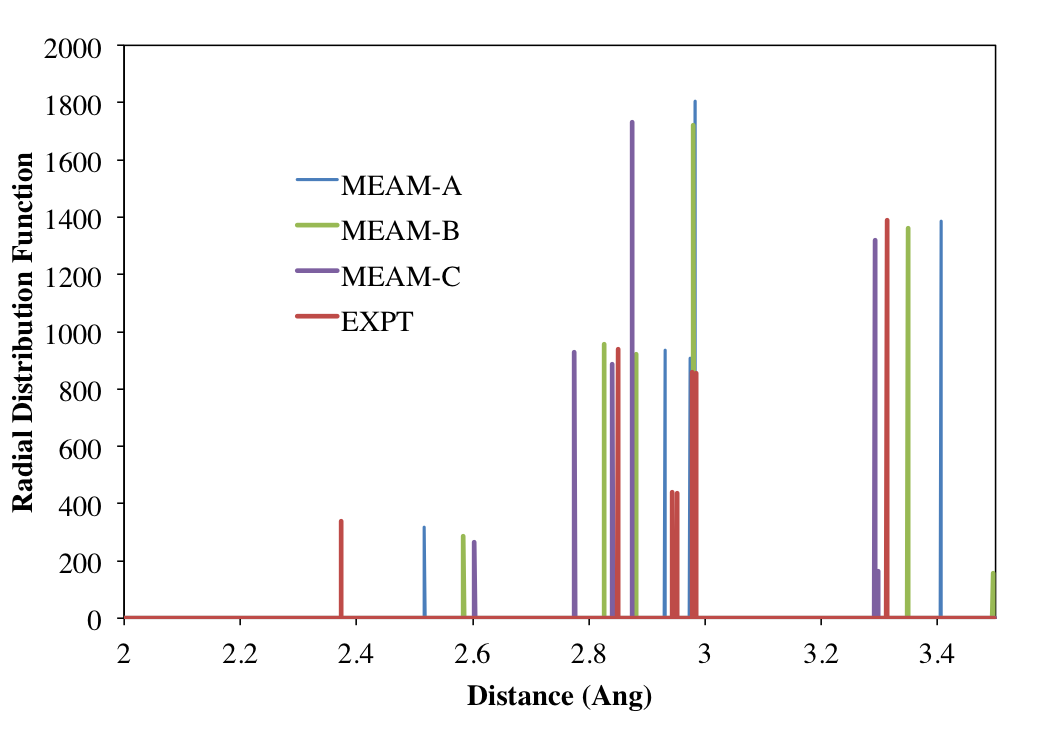
\includegraphics[width=0.8\textwidth]{rdf_image3.png}
    \caption{Radial distribution functions of U$_{3}$Si$_{2}$, comparing the MEAM predicted structures with the experimental structure.}\label{fig:benrdf}
\end{figure}

\FloatBarrier

Moving beyond the perfect crystal, the next step in testing the accuracy of the potential is to investigate point defects.  Single point defects (vacancy, interstitial, anti-site) were considered as a means of accommodating a change in stoichiometry.  The methodology for calculating point defect energetics is outlined in \cite{middleburgh2016}.  Point defect energies for the U$_{3}$Si$_{2}$ system are shown in Table \ref{tab:ben6} and compared to results from DFT \cite{middleburgh2016}.  Bound Schottky defects are also shown in Table \ref{tab:ben6}.  There exist two unique uranium sites in the U$_{3}$Si$_{2}$ structure.  Both U sites are investigated and denoted simply U1 (for the 2a site) or U2 (for the 4h site), as in Remschnig, $\textit{et al.}$ \cite{remschnig1992}.  The lowest energy interstitial site is determined via a molecular dynamics simulation performed at 1000 K that was then quenched down to 0 K and subsequently minimized.   In this way, the interstitial is able to reorient itself into the most preferable configuration.  Three unique simulations were performed to ensure the lowest energy configuration was obtained.  The bound Schottky defect consists of two U2 vacancies, one U1 vacancy and two Si vacancies, such that crystallographic accuracy is maintained, as well as the accurate chemical formula.  For the U-Si MEAM A potential, excellent agreement is observed for the formation energy of the U1 vacancy site, U interstitial and the Si interstitial.  Reasonable agreement is observed for the U2 vacancy and all anti-site defects.  The Si vacancy formation energy is substantially underestimated, and this likely leads to the bound Schottky defect energy being substantially underestimated as well.       The U-Si MEAM B potential performs similarly, with the notable differences being the much higher Si vacancy formation energy, although it is still below the DFT prediction.  This in turn leads to a higher Schottky defect formation energy.  The U-Si MEAM B potential overestimates the formation energy of the Si anti-site defect.  The U-Si MEAM C potential generally over-predicts the formation energy of defects.  However, good agreement is shown for the Si interstitial and the U1 and U2 anti-sites.  The U-Si MEAM C potential over-predicts the bound Schottky defect energy, in stark contrast to the other two potentials.  

\begin{table}[h!]
\caption{Properties of point defects in U$_{3}$Si$_{2}$ at 0 K.  Results from the MEAM U-Si potentials are compared to DFT calculations \cite{middleburgh2016}.  Units are eV.}\label{tab:ben6}
\begin{center}
\begin{tabular}{|c|c|c|c|c|}
     \hline
      &  DFT & U-Si MEAM A & U-Si MEAM B & U-Si MEAM C\\
     \hline
     U1 vac & 0.68 & 0.65 & 0.62 & 1.13\\
     U2 vac & 1.20 & 0.90 &  0.84 & 1.51\\
     Si vac & 1.59 & 0.57 & 1.20 & 2.17\\
     U int & 0.76 & 0.71 & 0.54 & 1.19\\
     Si int & 0.19 & 0.13 & 0.15 & 0.38\\
     U1 anti & 0.16 & 0.08 & 0.10 & 0.16\\
     U2 anti & 0.35 & 0.25 & 0.38 & 0.55\\
     Si anti & 0.35 & 0.34 & 0.68 & 1.67\\
     Schottky Bound & 7.57 & 5.21 & 5.74 & 11.6 \\
     \hline
\end{tabular}
\end{center}
\label{default}
\end{table}%

In order to ensure that the potentials are not restricted to studying only the U$_{3}$Si$_{2}$ phase, other phases, experimental and theoretical, were examined that were not included in the fitting procedure.  These include the FeB-USi, B1-USi, AlB$_{2}$-USi$_{2}$, L1$_{2}$-USi$_{3}$, U$_{3}$Si$_{5}$ phases and the L1$_{2}$, $\alpha$ and $\beta$ phases of U$_{3}$Si.  The results are shown in Figure \ref{fig:eform3}  for the energy per atom and in Figure \ref{fig:vol3} for the volume per atom across the composition range.  In Figure \ref{fig:eform3} for U-Si MEAM A, excellent agreement is observed for the U-rich portion of the composition range.  For U$_{3}$Si, U$_{3}$Si$_{2}$ and FeB-USi, formation energies are nearly identical to those from experiments \cite{berche2009}, and DFT calculations \cite{noordhoek2016}.  Also, the minimum is observed at USi$_{2}$ for the MEAM potential, which matches experiment, and the minimum is observed at U$_{3}$Si$_{5}$ (a distorted USi$_{2}$ structure with $\frac{1}{6}$ of the silicon sites vacant) for DFT, which shows reasonable agreement.  The energy of USi$_{2}$ is slightly lower than what would be consistent with the convex hull behavior shown in experiments \cite{berche2009}.  Significant variance is observed for the USi$_{3}$ and B1-USi structures, which are not included in the Figure \ref{fig:eform3} for the U-Si MEAM A potential.  These structures are deemed to be of less importance as they are either far away from the composition range of interest, in the case of USi$_{3}$, or not the low energy structure, in the case of B1-USi.  For the U-Si MEAM B potential, there exists a general over-prediction of the formation energy, although the general convex hull behavior is present.  Again, the USi$_{2}$ structure exhibits the lowest formation energy per atom, matching experiments.  As in the other potentials, greater deviation is present in the Si-rich regime.  For the U-Si MEAM C potential, excellent agreement is shown in the U-rich portion of the chart, matching the energies for U$_{3}$Si$_{2}$ and U$_{3}$Si.  Unlike the other two potentials, the lowest energy structure is the U$_{3}$Si$_{2}$ phase.  However, the general convex hull behavior is still present.  

In  Figure \ref{fig:vol3}, there exists a general negative parabolic trend in the volume predicted via the U-Si MEAM A potential as a function of composition, which matches the trends from DFT quite well.  The volume per atom is overestimated in the Si-rich portion of the composition range.  Per-atom volumes of U$_{3}$Si$_{2}$ and U$_{3}$Si agree very well.  Given that only U$_{3}$Si$_{2}$ was utilized as a fitting target and L1$_{2}$-U$_{3}$Si was utilized as a reference structure, there is considerable agreement across the entire composition spectrum when comparing MEAM predicted results to the results from DFT calculations.   The U-Si MEAM B potential exhibits the same behavior as the U-Si MEAM A potential for the the volume per atom, with excellent agreement in the U-rich composition range and over-prediction of the volume in the Si-rich composition regime.  The U-Si MEAM C potential even more closely matches the volume per atom predictions from DFT and measurements from experiments, while slightly under-predicting U$_{3}$Si$_{2}$ and over-predicting USi$_{3}$.

It should be noted that DFT (GGA without Hubbard U) calculations \cite{noordhoek2016} found the presence of another structure for U$_{3}$Si$_{2}$ that is lower in energy than the experimental structure.  This structure was destabilized by the addition of the Hubbard U term, which resulted in the correct prediction of the experimental structure as the ground state.  In order to ensure no such low energy structure exists in the MEAM potential energy landscape, this alternate U$_{3}$Si$_{2}$ structure was analyzed.  In order to ensure all possible transformations and relaxations were allowed, a molecular dynamics simulation was performed at 500 K, followed by a quench to 0 K and a subsequent minimization.  Throughout the entire relaxation process, each of the six components of the stress tensor are independently controlled.  The U-Si MEAM A potential finds this alternate structure to be 0.06 eV/at lower in energy than the experimental structure, matching DFT but not DFT+U or experiment.  The U-Si MEAM B potential finds his alternate structure to be 0.01 eV/at higher in energy than the experimental structure, matching DFT+U and experiment.  The U-Si MEAM C potential finds his alternate structure to be 0.09 eV/at higher in energy than the experimental structure.  The implications of these results will be discussed in greater detail later.

\begin{figure}[hbt]
	\centering
	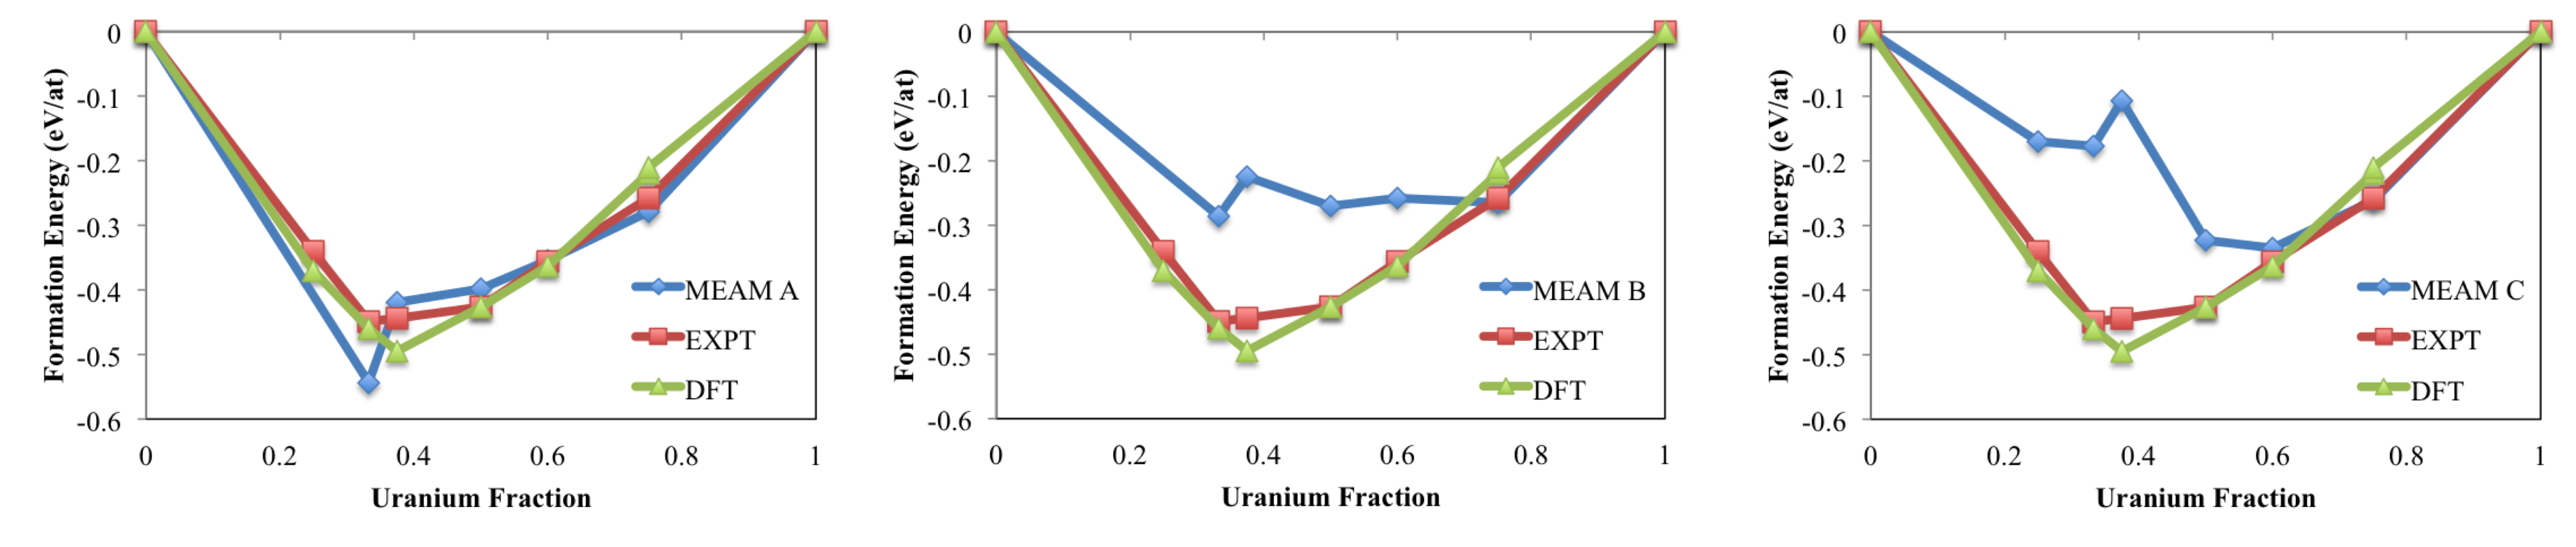
\includegraphics[width=\textwidth]{eform3.png}
    \caption{Formation energy per atom as a function of uranium concentration for a variety of phases in the U-Si system as calculated by the three MEAM potentials and compared to DFT calculations \cite{noordhoek2016} and experiments \cite{berche2009}.}\label{fig:eform3}
\end{figure}

 \begin{figure}[hbt]
	\centering
	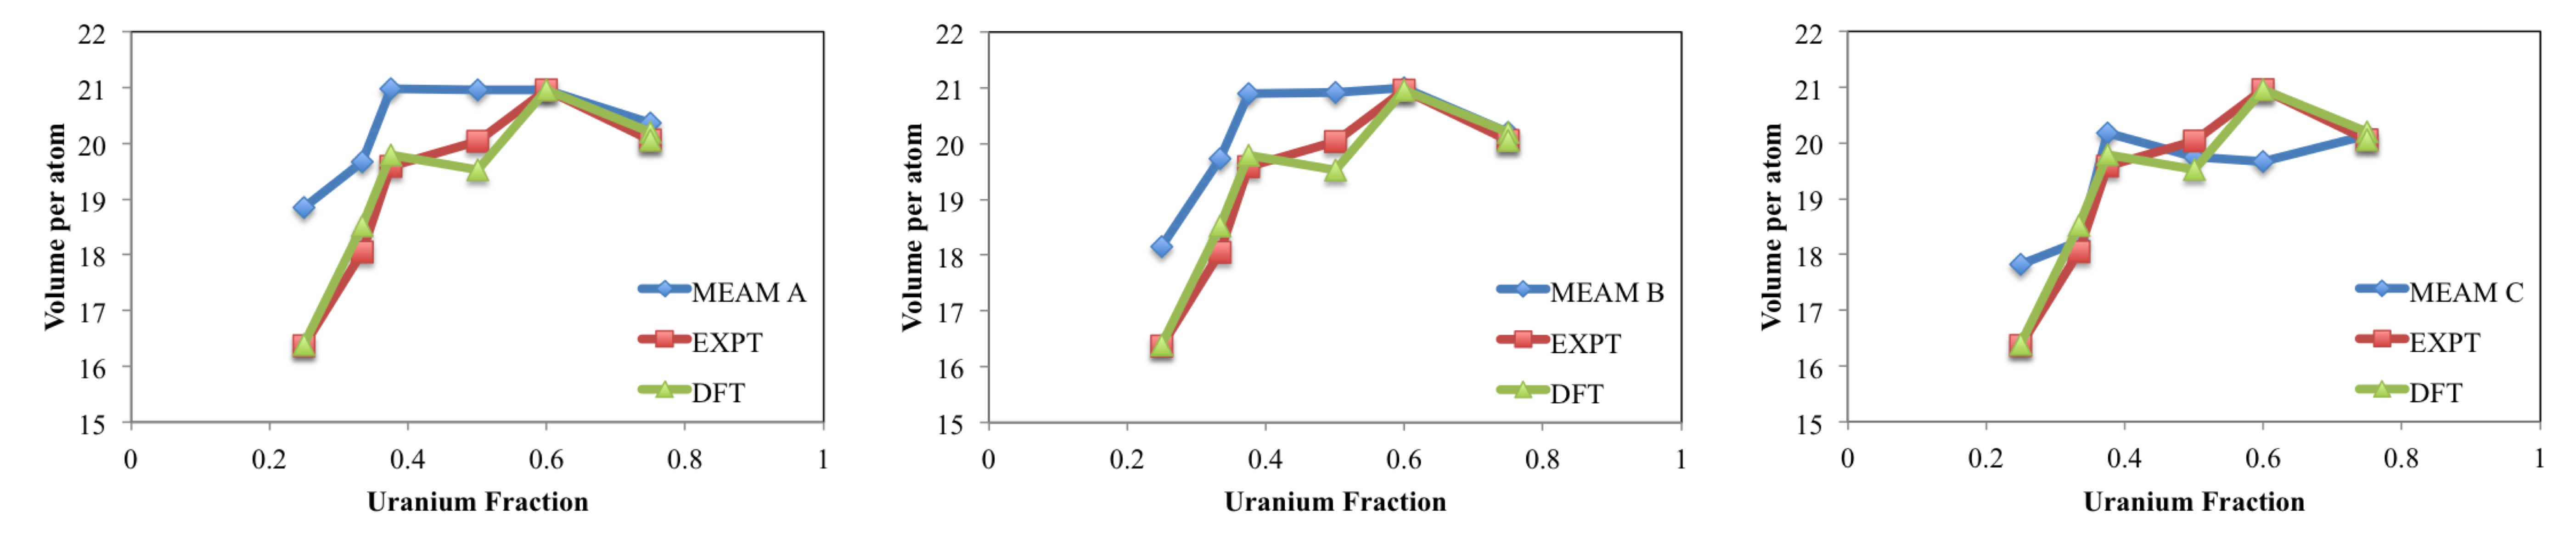
\includegraphics[width=\textwidth]{vol3.png}
    \caption{Volume per atom as a function of uranium concentration for a variety of phases in the U-Si system as calculated by the three MEAM potentials and compared to DFT calculations \cite{noordhoek2016} and experiments \cite{berche2009}.}\label{fig:vol3}
\end{figure}

\FloatBarrier

Although the ability to accurately predict the properties of a variety of crystal structures at 0 K is a critical step in the generation of a reasonable interatomic potential, being able to accurately model systems at non-zero temperatures is necessary to fully utilize the strength of molecular dynamics in branching the atomistic and mesoscopic time and length scales.  Thus, the nature of U$_{3}$Si$_{2}$ was examined as a function of temperature.  A 360 atom (3$\times$3$\times$4 unit cells) supercell is equilibrated at a given temperature in an NPT ensemble utilizing a Nose-Hoover barostat and a Langevin thermostat in the Gr{\o}nbech-Jensen-Farago \cite{gjf2013} formalism with a 1 fs timestep.  The damping parameters for the Nose-Hoover barostat and the Langevin thermostat are 0.1 and 0.01, respectively.  The target pressure is zero with the $\it{x}$, $\it{y}$ and $\it{z}$ components independently controlled. The systems are equilibrated for 100 ps, with energies and volumes determined by averaging over the final 50 ps of the simulation.  The total energy and total volume of the supercell as a function of temperature are displayed in Figure \ref{fig:temp}.  For all three potentials, it is observed that the structure is stable and behaves predictably as a function of temperature.   There are no observed obvious crystal structure changes or discontinuities suggesting potential instabilities.  The structure was visually confirmed to be U$_{3}$Si$_{2}$ throughout the temperature range investigated.  The normalized lattice constants are also analyzed as a function of temperature to ensure there exist no structural irregularities.  These are displayed in Figure \ref{fig:latticetemp}.  For all potentials, there is expansion of the $\it{a}$ and $\it{b}$ lattice constants in equal proportion as temperature increases, suggesting the tetragonal symmetry of the crystal structure is retained.  The $\it{c}$ lattice constant shows very different behavior depending on the potential.  For the U-Si MEAM A, compression is observed as temperature increases, and thus a decrease in the $\it{c/a}$ ratio as temperature increases.  For the U-Si MEAM B potential, the $\it{c}$ lattice constant shows very minimal expansion, with a slight negative parabolic trend as temperature increases, and thus a decrease in the $\it{c/a}$ ratio as temperature increases.  For the U-Si MEAM C potential, the $\it{c}$ lattice constant shows much more dramatic expansion with temperature than the $\it{a}$ lattice constant.  This results in an increase in the $\it{c/a}$ ratio as temperature increases, in contrast to the two other potentials.  

From Figure \ref{fig:temp}, the thermal expansion can be extracted.  The calculated MEAM average linear thermal expansion from 200 K to 1200 K is 18.6x10$^{-6}$ K$^{-1}$, 17.6x10$^{-6}$ K$^{-1}$ and 16.0x10$^{-6}$ K$^{-1}$ for the U-Si MEAM A, U-Si MEAM B and U-Si MEAM C, respectively.  The experimental linear thermal expansion is 14-17x10$^{-6}$ K$^{-1}$ from Shimizu \cite{shimizu1965} and 16.1x10$^{-6}$ K$^{-1}$ from White \cite{white2015}.  This is remarkable agreement across all three potentials given that this was not included into the fitting procedure.  

The molar heat capacity, given by equation \ref{eq:cp}, was calculated at 400 K for comparison with White, et al. \cite{white2015}.  The calculated values from the MEAM potentials are 120.7 J/mol-K, 117.3 J/mol-K and  61.7 J/mol-K for the U-Si MEAM A, U-Si MEAM B and U-Si MEAM C, respectively.  This quantity for U-Si MEAM A and U-Si MEAM B compares very favorably to the Dulong-Petit value of 125 J/mol-K and is slightly less than the experimental value of White, et al., which is 150 J/mol-K.  The value from the U-Si MEAM C potential significantly underestimates the experimental measurements.  It should be reiterated that this thermo-physical property was not included into the fitting procedure, and thus this is considered excellent agreement to both theory and experiment.  Regretfully, relatively little other experimental data exists for comparison.  

\begin{equation}
\label{eq:cp}
C_{P} = \left(\frac{\delta H}{\delta T}\right)_{P}
\end{equation}

 \begin{figure}[hbt]
	\centering
	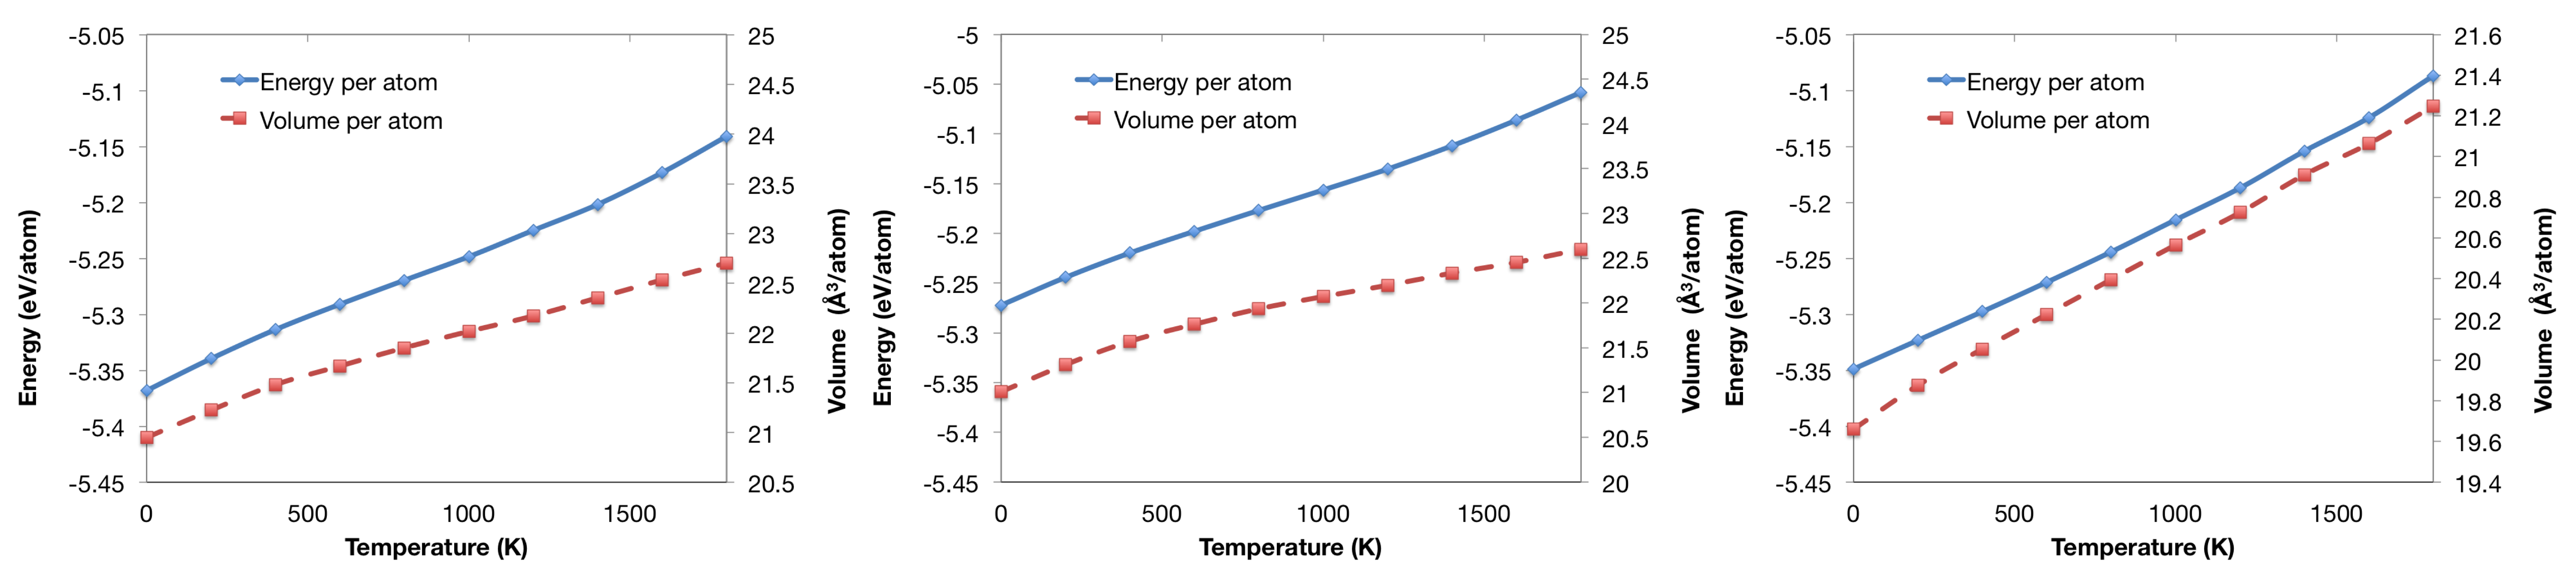
\includegraphics[width=\textwidth]{u3si2temp3.png}
    \caption{Energy per atom and volume per atom of U$_{3}$Si$_{2}$ as a function of temperature for each of the three U-Si MEAM potentials.  Panels from left to right: U-Si MEAM A, U-Si MEAM B, U-Si MEAM C.}\label{fig:temp}
\end{figure}

\begin{figure}[hbt]
	\centering
	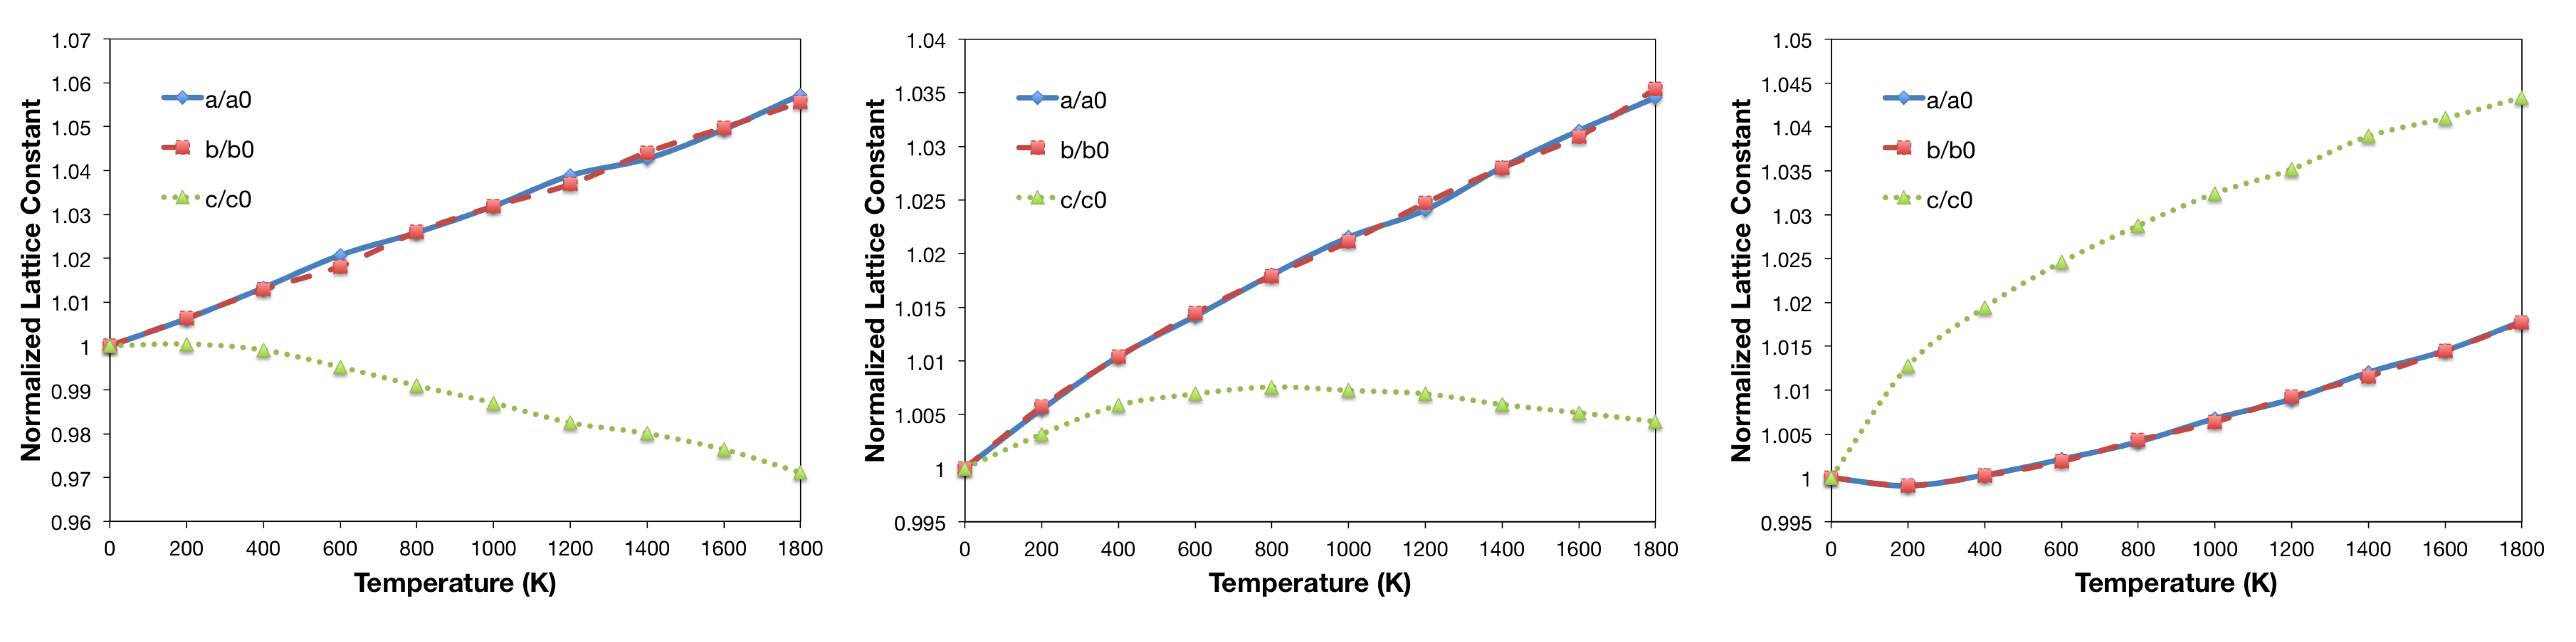
\includegraphics[width=\textwidth]{latticetemp3.png}
    \caption{Variation of normalized lattice constants of U$_{3}$Si$_{2}$ as a function of temperature for each of the three U-Si MEAM potentials.  Panels from left to right: U-Si MEAM A, U-Si MEAM B, U-Si MEAM C.}\label{fig:latticetemp}
\end{figure}

The high temperature regime was investigated by calculating the melting point of U$_{3}$Si$_{2}$ using each potential.  In order to determine the melting point, a two-phase system was constructed consisting of crystal and liquid phases, as in Figure \ref{fig:twophase}.  This system was constructed by holding half of the supercell at a temperature known to be below the melting point and super-heating the other half of the supercell to induce melting.  This system is then evolved at a temperature near the melting point, and the two-phase interface is tracked.  Advancement of the liquid phase into the crystal phase indicates that the system is at a temperature above the melting point.  The system was investigated in increments of 50 K in order to determine a general temperature regime for the melting point of U$_{3}$Si$_{2}$.  The calculated melting point is approximately 1250 K, 1575 K, 1825 K for the U-Si MEAM A, U-Si MEAM B and U-Si MEAM C, respectively.  The experimental melting point is 1938 K \cite{berche2009}.  The only potential that approaches an accurate melting point of U$_{3}$Si$_{2}$ is the U-Si MEAM C, while U-Si MEAM A and U-Si MEAM B significantly underestimate the melting point.  

\begin{figure}[hbt]
	\centering
	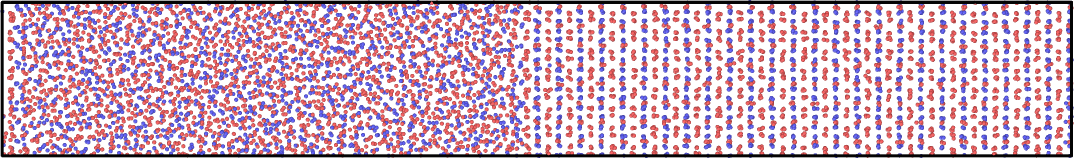
\includegraphics[width=\textwidth]{two_phase2.png}
    \caption{Two-phase system employed in the determination of the melting point of U$_{3}$Si$_{2}$.}\label{fig:twophase}
\end{figure}

\FloatBarrier

As a nuclear fuel, it is necessary that this potential be able to model U$_{3}$Si$_{2}$ under irradiation.  In order to test the ability of the potentials to model radiation damage, a 1 keV cascade is investigated.   The MEAM potentials are splined to a Ziegler-Biersack-Littmark (ZBL) \cite{zbl} potential in the standardized method implemented into LAMMPS.  A 20,000 atom supercell (10$\times$10$\times$20 unit cells) is equilibrated at 500 K for 100 ps in an NPT ensemble with a target pressure of 0 GPa.  In an NVT ensemble, a U1 atom is given additional kinetic energy in the $[$135$]$ direction.  The timestep is reduced to 0.2 fs and the cascade is allowed to evolve for 12 ps.  The residual damage is then evolved at 500 K for 1 ns utilizing a 2 fs timestep.  The state of the cascade and residual damage for the U-Si MEAM A potential is displayed in Figure \ref{fig:ben6} at three different times throughout the simulation.  It is observed that the crystal structure is stable and there exists a thermal spike and subsequent annealing stage.  At 0.4 ps after cascade initiation, Wigner-Seitz analysis via Ovito \cite{ovito} shows that there exist 68 Frenkel pairs; there exist 28 Frenkel pairs after 12 ps; there exist 17 Frenkel pairs after 1 ns.  By investigating defects on each species sublattice, it can be determined the general nature of the defects generated via this specific cascade.  Looking strictly at the uranium sublattice, 23 Frenkel pairs exist.  Looking strictly at the silicon sublattice, 23 Frenkel pairs exist.  This gives a total of 46 Frenkel pairs.  It can thus be determined that in the total system there exist 28 Frenkel pairs and 18 anti-site defects, with the same number of defects on each sublattice.  It can be concluded that this potential is displaying reasonable behavior under irradiation and the nature and number of defects can be readily determined.  It should be noted that this is not intended to be a full radiation damage study, but simply an example that this potential produces reasonable radiation damage behavior.  Radiation damage studies are certainly warranted in the future.  Cascade investigations were performed for each of the other two potentials, yielding similar results.  

 \begin{figure}[bt]
	\centering
	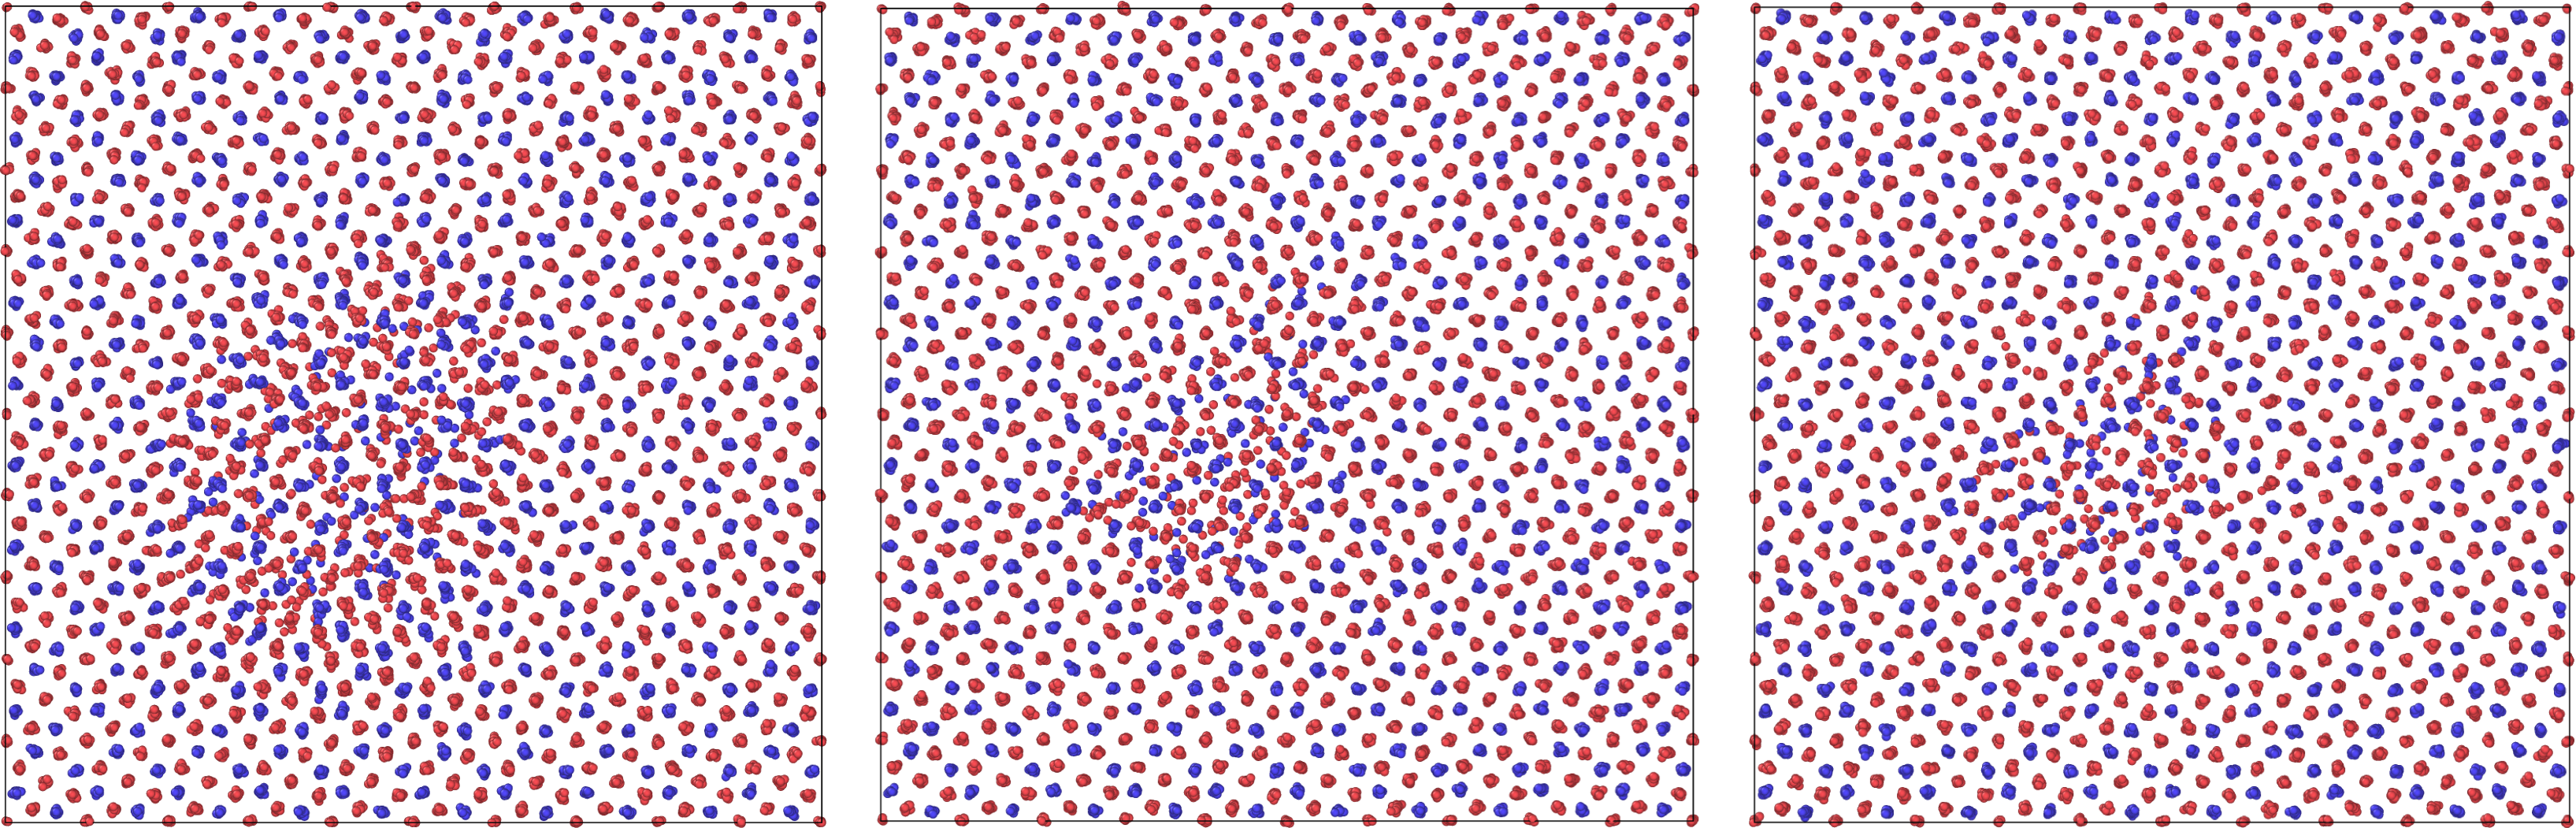
\includegraphics[width=\textwidth]{cascade_total.png}
    \caption{1 keV cascade behavior of U$_{3}$Si$_{2}$ at 500 K.  The left-most panel is 0.4 ps after cascade initiation; the middle panel is 12 ps after cascade initiation; the right-most panel is 1 ns after cascade initiation.}\label{fig:ben6}
\end{figure}

\begin{comment}
 \begin{figure}[bt]
	\centering
	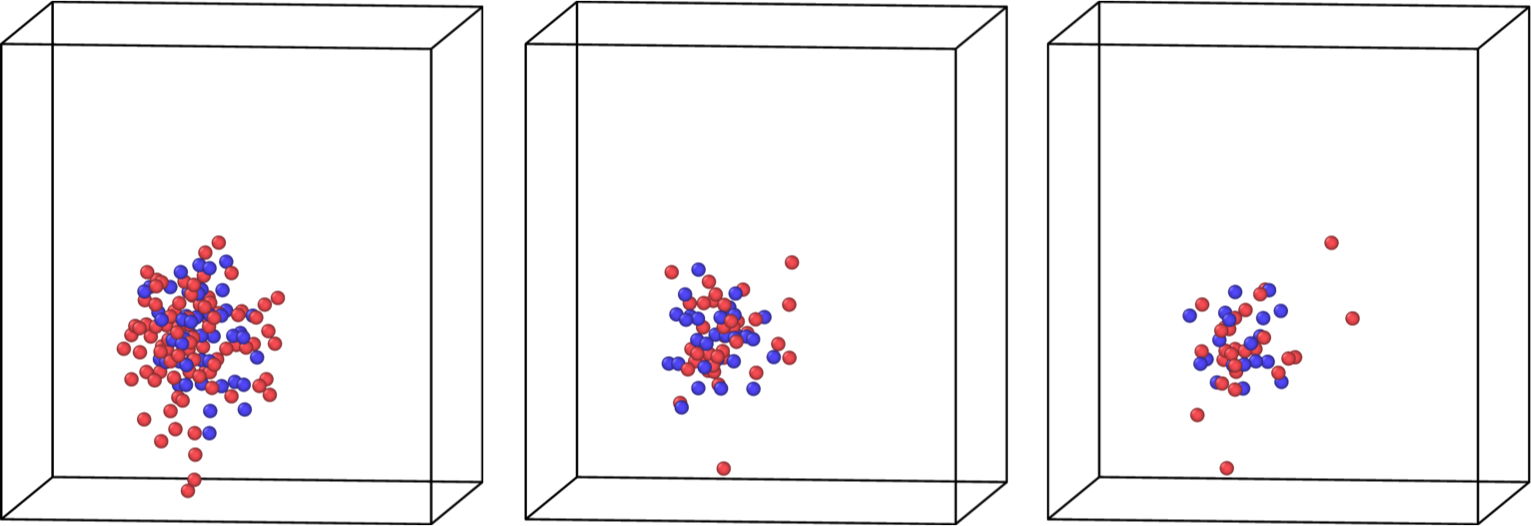
\includegraphics[width=\textwidth]{alt_cascadeTOTAL.png}
    \caption{1 keV cascade behavior of U$_{3}$Si$_{2}$ at 500 K.  The left-most panel is 0.4 ps after cascade initiation; the middle panel is 12 ps after cascade initiation; the right-most panel is 1 ns after cascade initiation.}\label{fig:ben6}
\end{figure}
\end{comment}

\FloatBarrier

Another microstructural feature of interest is free surfaces.  To investigate the nature of free surfaces, two systems are created to investigate both the (100) free surface and the (001) free surface (there exist multiple possible terminations, but in this work all terminuses are created at unit cell boundaries).  For the (100) free surface, a system supercell of 16x6x8 unit cells (7728 atoms) was generated with a vacuum region of 4 unit cells in the x direction.  For the (001) free surface, a system supercell of 6x6x16 unit cells (5976 atoms) was generated with a vacuum region of 4 unit cells in the z direction.  Both longer and shorter systems were analyzed with more vacuum region and it was determined that this setup provided an accurate determination of the surface energies.  The system with free surfaces is equilibrated in an NPT ensemble at 500 K for 100 ps and the average energy is determined over the final 50 ps of the simulation.  The relaxed structures of the (100) and (001) free surfaces are shown in Figure \ref{fig:ben7} and Figure \ref{fig:ben8}, respectively, using the U-Si MEAM B potential.  The first thing to notice is that the bulk structure remains stable and retains its crystal symmetry.  The surface energies are determined by equation \ref{eq:surface}

\begin{equation}
\label{eq:surface}
E_{surf}= \frac{(E^{*} - E)}{2*A} * N
\end{equation}

where $\it{E^{*}}$ is the energy per atom of the system with two free surfaces, $\it{E}$ is the energy per atom of the perfect crystal U$_{3}$Si$_{2}$, $\it{A}$ is the area of a free surface (multiplied by two because two free surfaces are present in the system) and $\textit{N}$ is the number of atoms in the system with two free surfaces.  The resultant energy for the (100) surface is 1.09 J/m$^{2}$ and the (001) surface energy is 1.21 J/m$^{2}$ (for the U-Si MEAM B potential).  A prior DFT study investigated free surfaces in U$_{3}$Si$_{2}$ \cite{anl_report}.  The surface energy was found to vary from 1.16 J/m$^{2}$ to 1.48 J/m$^{2}$.  In this study, the (100) surface had a surface energy of 1.48 J/m$^{2}$, while the (001) surface had a surface energy of 1.43 J/m$^{2}$.  The nature of the lowest energy surface was not reported.  Both the U-Si MEAM A and U-Si MEAM C potentials produce similar results, with the U-Si MEAM A potential yielding surface energies slightly lower with respect to the U-Si MEAM B potential and the U-Si MEAM C potential yielding surface energies slightly higher.  Given that the physical nature of the surfaces as predicted by the MEAM potentials is reasonable combined with the calculation of reasonable surface energies, it is suggested that the interatomic potentials performs adequately for free surfaces in U$_{3}$Si$_{2}$.  Of course, further experimental and computational investigations are required for validation of this predicted surface behavior.  

\begin{figure}[bt]
	\centering
	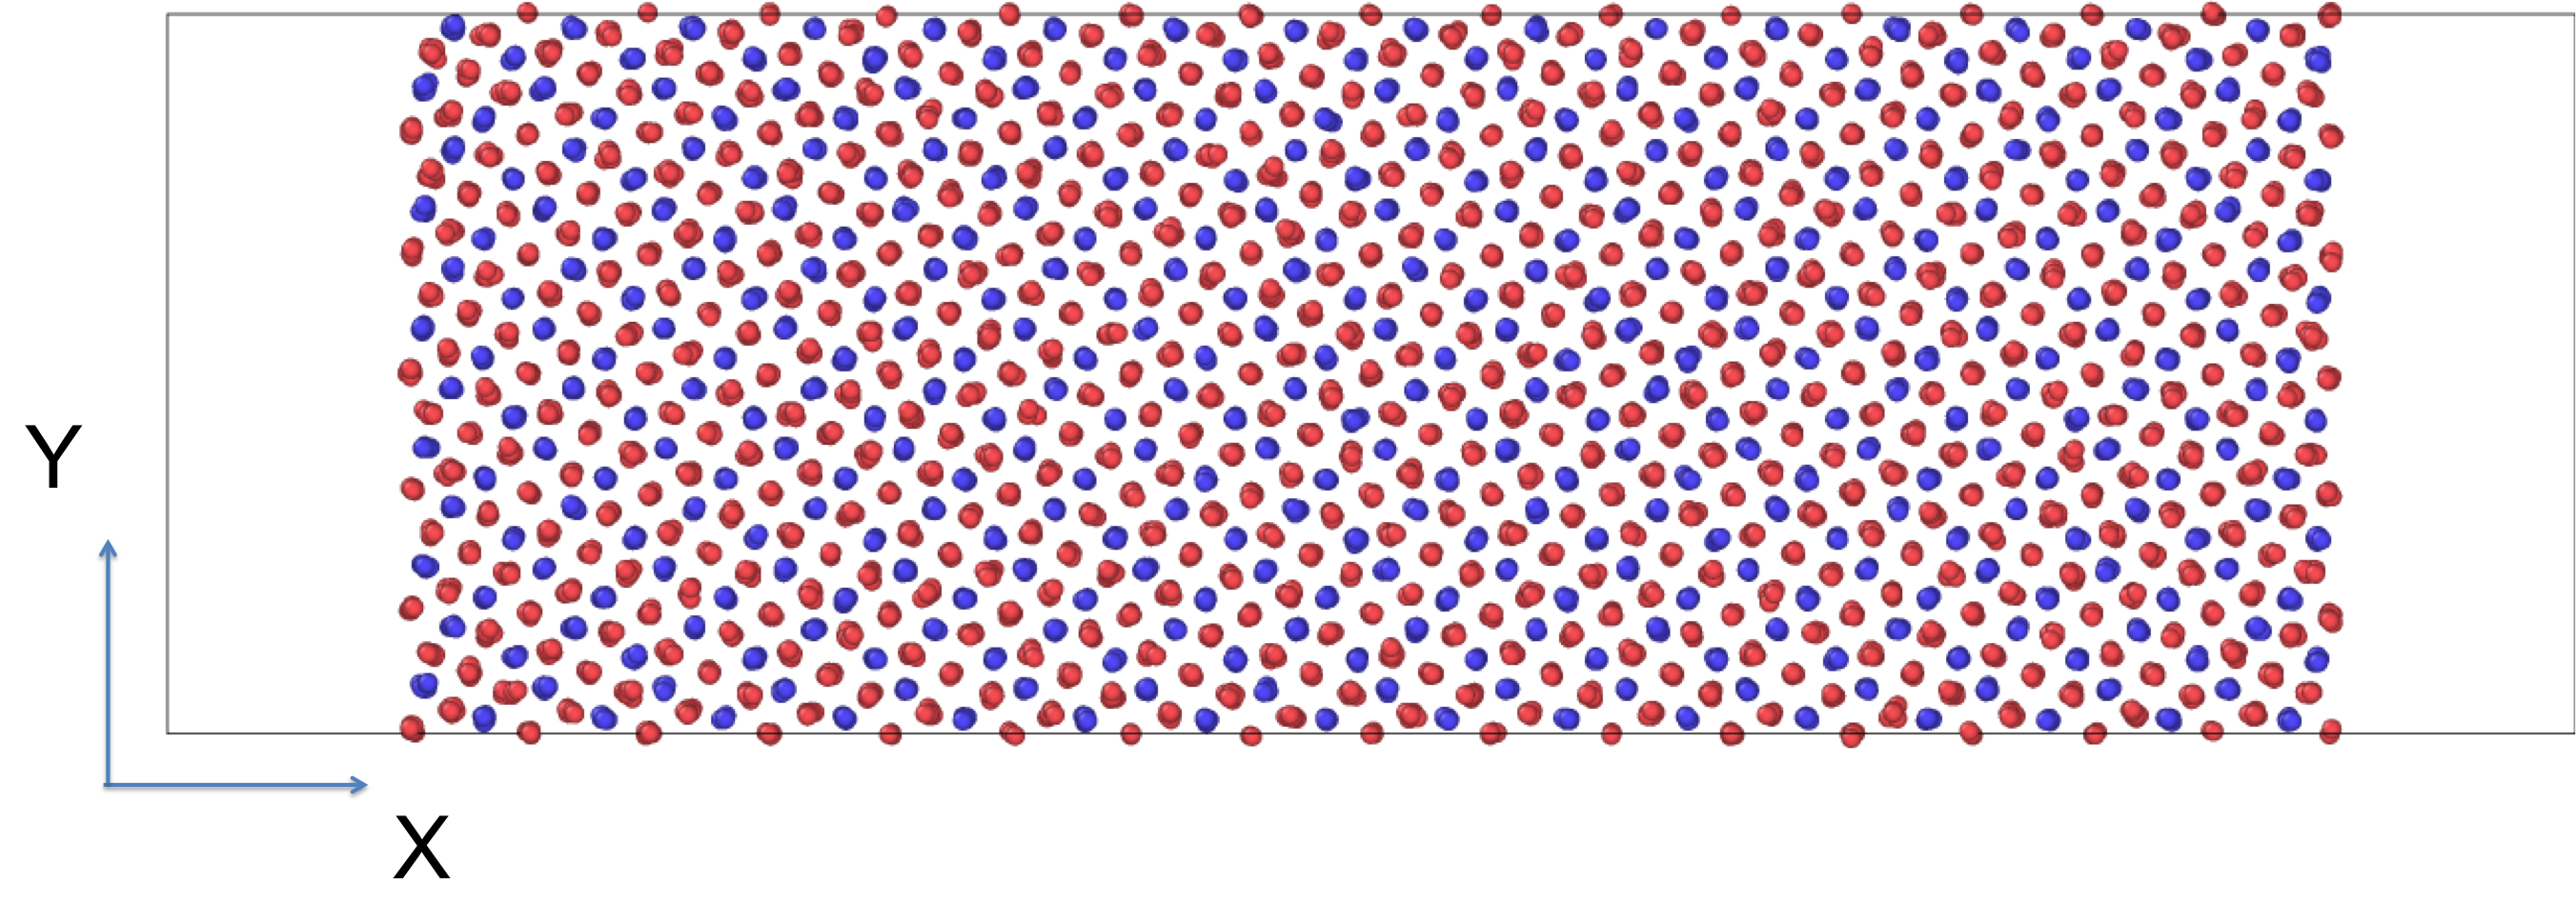
\includegraphics[width=0.9\textwidth]{100surfaceB.png}
    \caption{(100) free surface of U$_{3}$Si$_{2}$ at 500 K after a 100 ps relaxation.}\label{fig:ben7}
\end{figure}

\begin{figure}[bt]
	\centering
	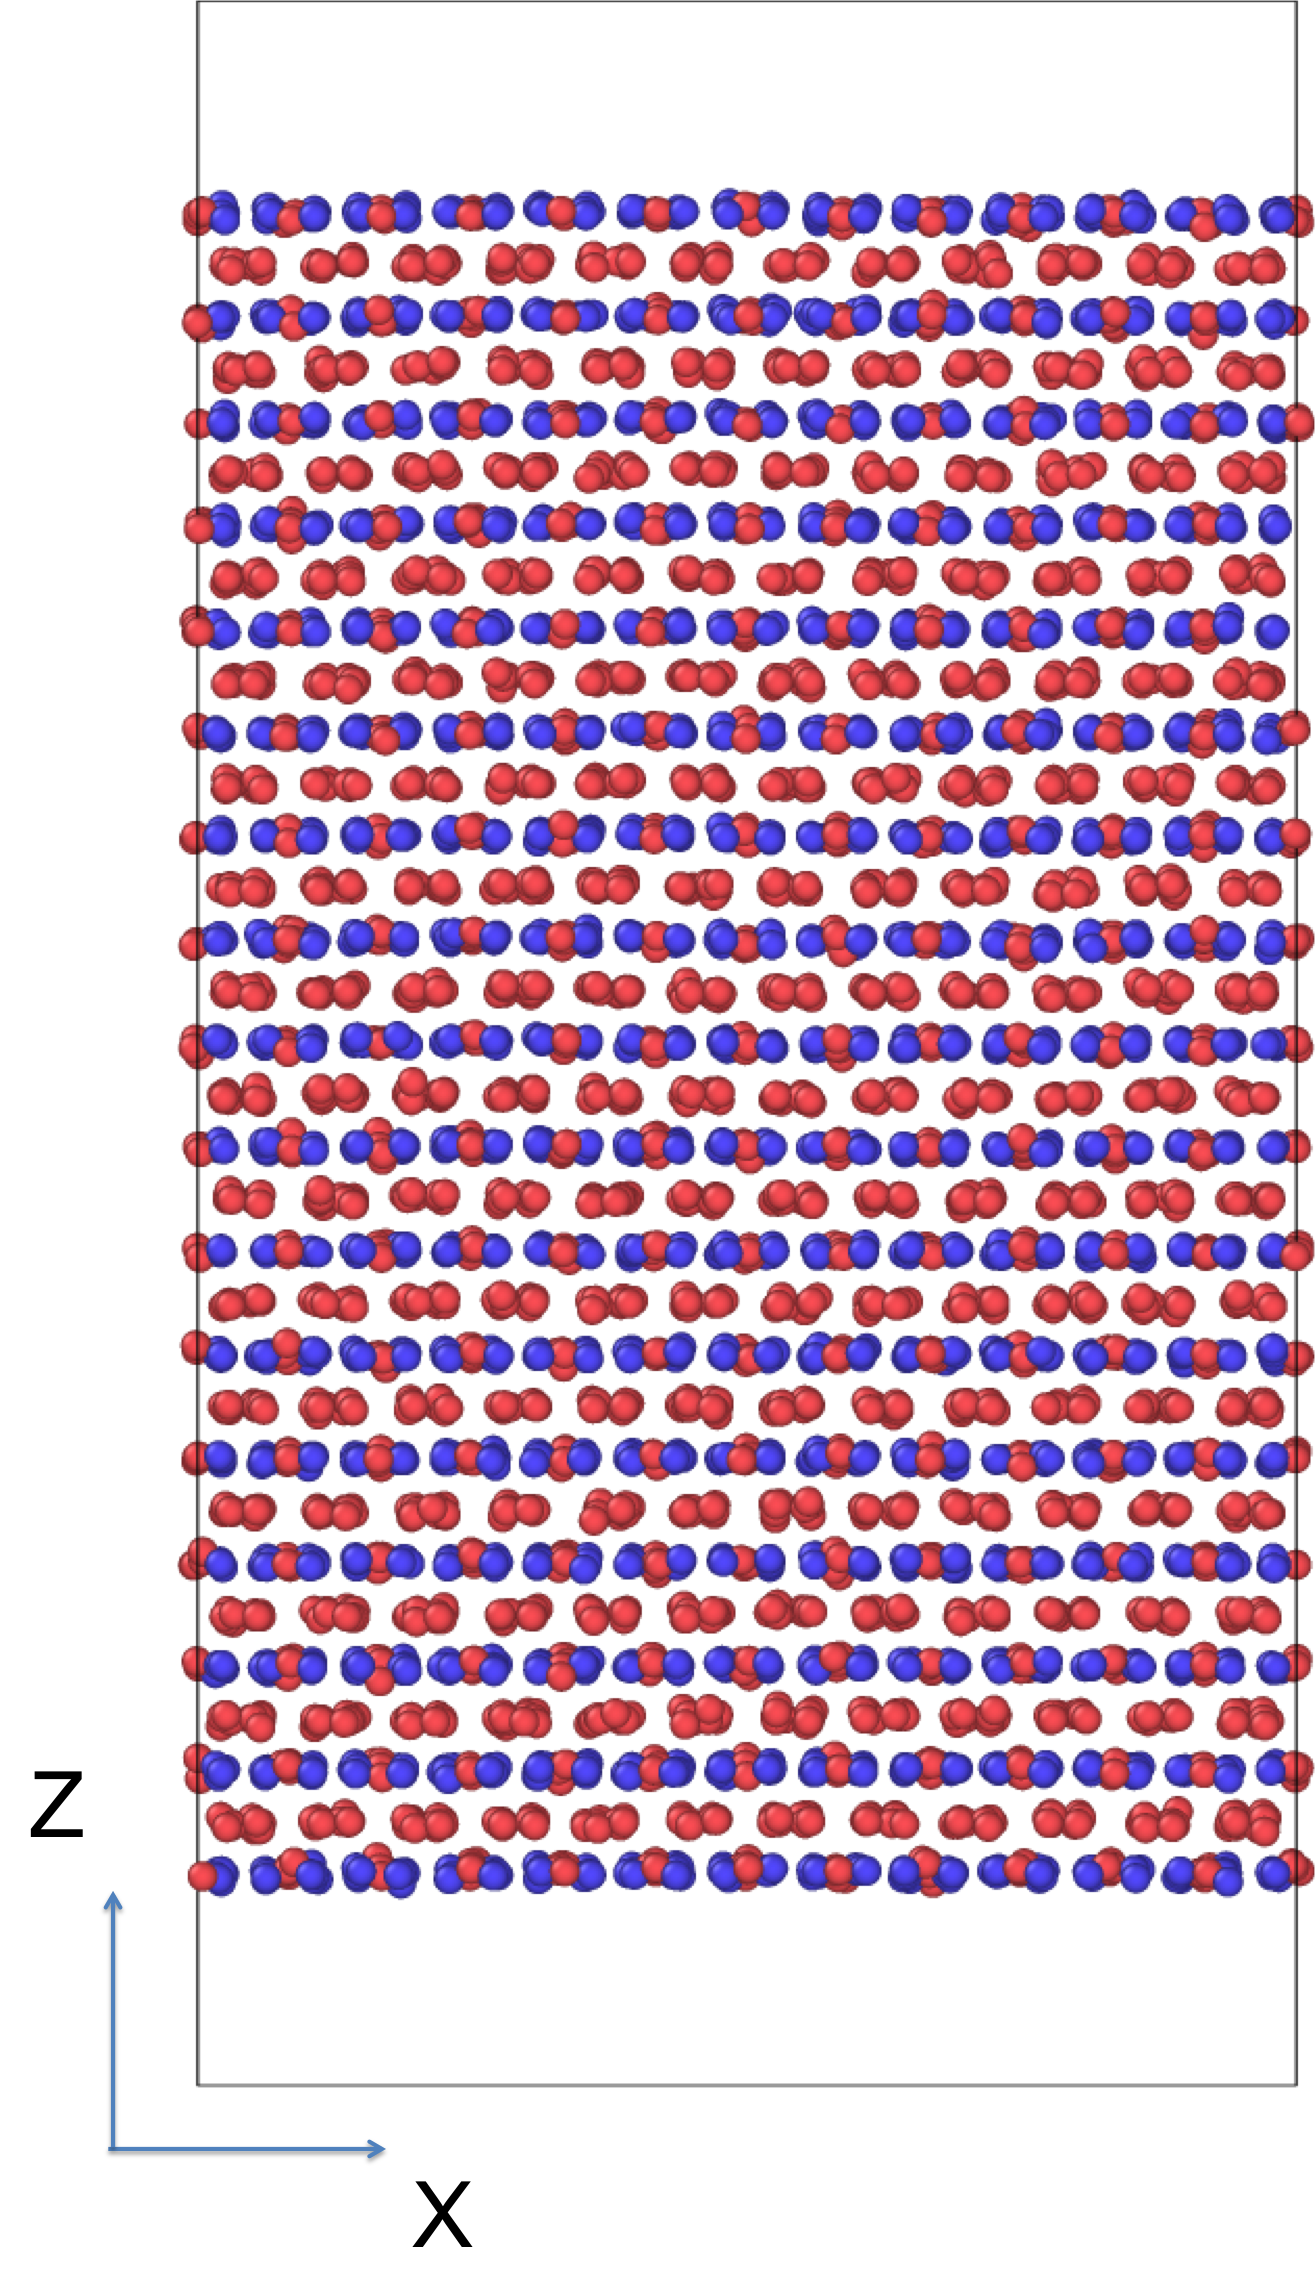
\includegraphics[width=0.4\textwidth]{001surfaceB.png}
    \caption{(001) free surface of U$_{3}$Si$_{2}$ at 500 K after a 100 ps relaxation. }\label{fig:ben8}
\end{figure}

To further investigate the performance of the potential, as well as to calculate an average surface energy, a void is introduced into an equilibrated U$_{3}$Si$_{2}$ system, and then further relaxed.  The system with a void is equilibrated in an NPT ensemble at 500 K for 100 ps and the average energy is determined over the final 50 ps of the simulation.  It is observed that voids from a radius of 4 {\AA} up to 32 {\AA} are stable within U$_{3}$Si$_{2}$ up to 100 ps (when simulations were terminated).   A representative void with a radius of 25 {\AA} is shown in Figure \ref{fig:void}.  No void collapse is observed, no crystal structure collapse or distortion is observed, but minimal void surface reconstruction does occur.  This further reinforces the suitability and stability of the potential for non-equilibrium systems.  The void surface energy is determined via equation \ref{eq:void}.

\begin{equation}
\label{eq:void}
E_{surf}= \frac{(E^{*} - E)}{A} * N
\end{equation}

where $\it{E^{*}}$ is the energy per atom of the system with a void, $\it{E}$ is the energy per atom of the perfect crystal U$_{3}$Si$_{2}$, $\it{A}$ is the surface area of the void and $\textit{N}$ is the number of atoms in the system with a void.  The void size is increased, along with system size, until the void surface energy converged for each potential.  The representative void surface energies are 0.7$\frac{J}{m^{2}}$, 1.0$\frac{J}{m^{2}}$ and 1.7$\frac{J}{m^{2}}$ for the U-Si MEAM A, U-Si MEAM B and U-Si MEAM C, respectively.

\begin{figure}[bt]
	\centering
	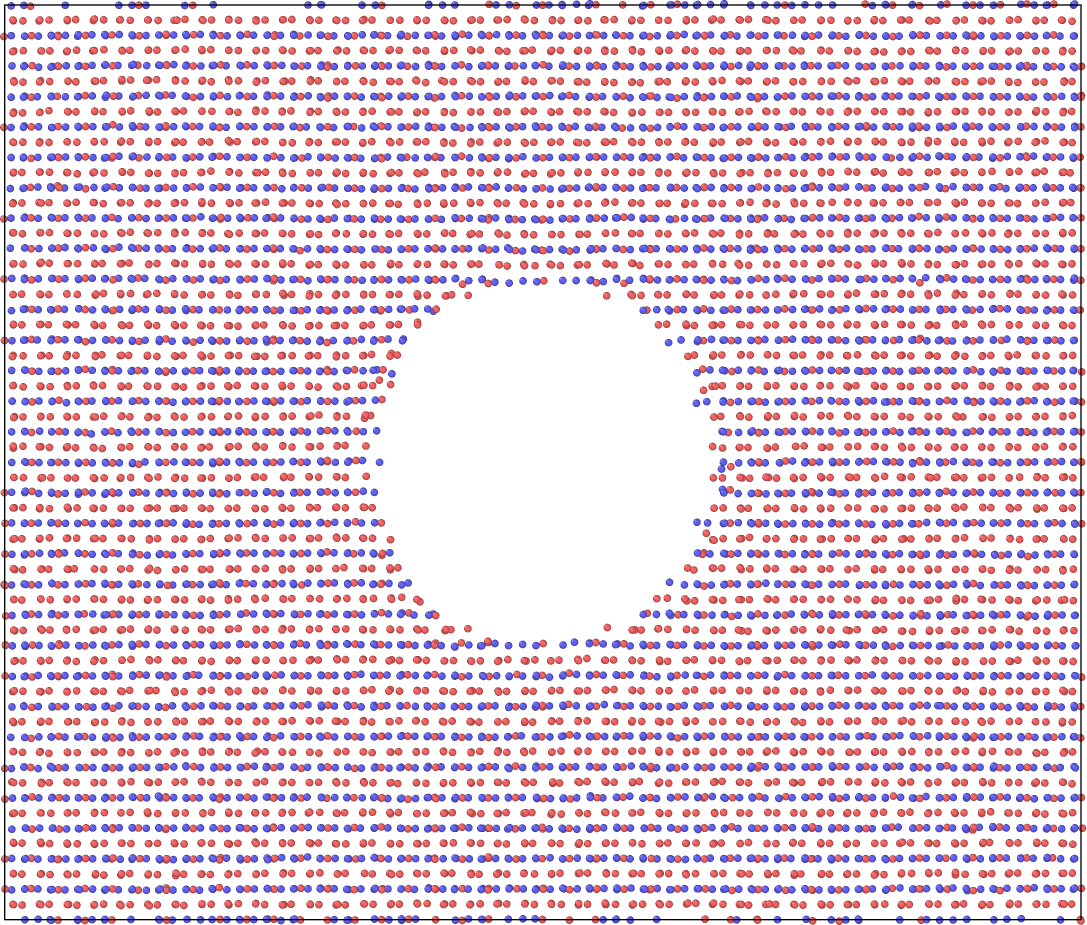
\includegraphics[width=0.8\textwidth]{void3.png}
    \caption{2D projection of a 3D slice through the a U$_{3}$Si$_{2}$ supercell at 500 K containing a void with a radius of 25 {\AA}.  }\label{fig:void}
\end{figure}

\FloatBarrier
\clearpage

\section{Discussion}

The above assessment shows that each of the potentials perform satisfactorily for the U$_{3}$Si$_{2}$ phase, but with each potential showing specific strengths and weaknesses.   The U-Si MEAM A potential is the most accurate with regards to cohesive energy, volume per atom, and elastic constants at 0 K.  Some defect properties are well re-produced, but the Si vacancy and Schottky defect energy are greatly underestimated.  This most likely leads to the dramatic underestimation of the melting point via the U-Si MEAM A potential.  This potential also most closely reproduces the shape and magnitude of the formation energy as a function of composition over the entire U-Si composition range.  One final issue is the prediction of the theoretical phase of U$_{3}$Si$_{2}$ suggested by \cite{noordhoek2016} at a lower energy than the experimental structure.  Although a direct phase change would be incredibly difficult, in extreme environments this phase could present itself.  Thus, this potential is most well suited for low temperature studies of U$_{3}$Si$_{2}$ and other phases in the U-rich portion of the U-Si composition regime.  

The U-Si MEAM B potential shows the most accuracy with regards to point defect energetics.  This potential shows good accuracy for all defects studied, excepting an underestimation of the bound Schottky defect formation energy.  The highest variation from DFT for elastic constant calculations is observed for the U-Si MEAM B potential, as well as an overestimation of the formation energy of U$_{3}$Si$_{2}$.  This potential shows good behavior across the U-Si composition spectrum, but with consistently higher predicted formation energies.  The predicted melting point is higher than that of U-Si MEAM A, but still underestimates the experimental melting point by 400 K.  This potential is best suited for low and intermediate temperature investigations, particularly those involving isolated point defects.  

The U-Si MEAM C potential exhibits the best high temperature behavior.  This potential comes closest to the experimental melting point and exhibits the most accurate thermal expansion (although all potentials express quite good predictions of thermal expansion).  This potential generally overestimates the defect formation energies, excepting the Si interstitial and the two U anti-site defects.  This potential most accurately describes the volumes of various U-Si phases across the composition regime, but only accurately describes the energetics in the U-rich region.  This potential is best suited for high temperature simulations of U$_{3}$Si$_{2}$.  

Again, each potential presents its own strengths and weaknesses and the suitable potential should be chosen based on the specific nature of the simulation.  Finally, these potentials are not intended for investigation of liquid phase U$_{3}$Si$_{2}$, as this was not taken into account in the fitting procedure nor fully explored by the authors.  

Given the complex nature of the crystal structure of U$_{3}$Si$_{2}$, the inherent difficulties associated with the development of atomic potentials for pure uranium, let alone uranium-alloys, it is the opinion of the authors that three suitable interatomic potentials to describe the U-Si system have been developed.  Provided that the scientific community is continually gaining more knowledge on U-Si alloys via experimentation and first principles examinations, future refinement of the potentials should be undertaken once more atomistic and fundamental property information has been gathered.  

\section{Conclusion}

MEAM interatomic potentials were developed for the U-Si system.  The potentials accurately describe 0 K properties of the primary phase of interest (U$_{3}$Si$_{2}$), including formation energy, lattice constants, elastic constants and several point defect properties.  The potentials can also reasonably predict properties of a variety of U-Si phases across the composition spectrum.  The predicted thermal expansion and heat capacity compare excellently to reported experimental values.  The interatomic potentials were tested by investigating the behavior of U$_{3}$Si$_{2}$ under a 1 keV cascade, with free surfaces and in the presence of a void.  The potentials behave in a reasonable manner in each of these three non-equilibrium cases.  These potentials can serve as a tool to branch experiments and recent first principles calculations to future longer time and larger length scale simulations.  

\section{Acknowledgments}
This work is supported by the U.S. Department of Energy, Office of Nuclear Energy, Nuclear Energy Advanced Modeling and Simulation (NEAMS) Accident Tolerant Fuel High-Impact-Problem Program. This manuscript has been authored by Battelle Energy Alliance, LLC under Contract No. DEAC07-05ID14517 with the U.S. Department of Energy. The United States Government retains and the publisher, by accepting the article for publication, acknowledges that the United States Government retains a nonexclusive, paid-up, irrevocable, world-wide license to publish or reproduce the published form of this manuscript, or allow others to do so, for United States Government purposes.  Los Alamos National Laboratory, an affirmative action/equal opportunity employer, is operated by Los Alamos National Security, LLC, for the National Nuclear Security Administration of the U.S. Department of Energy under Contract No. DE-AC52-06NA25396.  This research made use of the resources of the High Performance Computing Center at Idaho National Laboratory, which is supported by the Office of Nuclear Energy of the U.S. Department of Energy and the Nuclear Science User Facilities under Contract No. DE-AC07-05ID14517.

\begin{comment}
\begin{appendix}
\section{Calculation of point defect energies in U$_{3}$Si$_{2}$}
Consider a base alloy A$_{x0}$B$_{1-x0}$ and energy per atom e$_{0}$ and a second phase with concentration of A$_{x\phi}$B$_{1-x\phi}$ and energy per atom e$_{\phi}$.  The energy per atom e$_{2phase}$ as function of composition is given by:

\begin{equation}
\label{eq:def1}
e_{2phase}(x)=\frac{x-x_{0}}{x_{\phi}-x_{0}}e_{\phi} + \frac{x_{\phi}-x}{x_{\phi}-x_{0}}e_{0} 
\end{equation}

Consider an A defect in the base alloy that changes stoichiometry, e.g., vacancy (V) (remove A atom), interstitial (I) (add A atom), or anti-site defect (AS) (add A atom and remove B atom).  We are interested in the energetics of a dilute solution of defects, but can conveniently calculate defect energies in only small 3D periodic systems.  Consider a small system with N atoms of base alloy with one defect and supercell energy E$_{d}$.  The number of atoms in this cell, N$_{d}$, is given by:

\begin{equation}
\label{eq:def2}
N_{d} = N + i_{d}
\end{equation}

where i$_{d}$ is the change in atoms with defect, e.g., i$_{d}$=1,0,-1 for the interstitial, anti-site defect, and vacancy respectively.  The number of A atoms in this cell, N$_{dA}$, is given by:

\begin{equation}
\label{eq:def3}
N_{dA} = x_{0}N + A_{d}
\end{equation}

where 

\begin{equation}
\label{eq:def4}
A_{d} = \begin{cases}
    1       & \quad d = I \\
    1       & \quad d = AS\\
    -1      & \quad d = V\\
  \end{cases} 
\end{equation}

The concentration in the cell x$_{d}$ is given by:

\begin{equation}
\label{eq:def5}
x_{d}=\frac{N_{dA}}{N_{d}} 
\end{equation}

The defect formation energy per cell may be defined as

\begin{equation}
\label{eq:def6}
E_{defect} = E_{d} - N_{d}e_{2phase}(x_{d})
\end{equation}

A convenient way to compare energies is to use atomic energies. We can express the energy of the 2-phase system as

\begin{equation}
\label{eq:def7}
e_{2phase}(x_{A}) = e_{A}x_{A} + e_{B}(1-x_{A})
\end{equation}

It is convenient to determine E$_{A}$ and E$_{B}$ by using the energies of the two phases.

\begin{equation}
\label{eq:def8}
e_{0} = e_{A}x_{0} + e_{B}(1-x_{0})
\end{equation}	 

\begin{equation}
\label{eq:def9}
e_{\phi} = e_{A}x_{\phi} + e_{B}(1-x_{\phi})
\end{equation}

which results in

\begin{equation}
\label{eq:def10}
e_{A}=\frac{e_{0}(1-x_{\phi})-e_{\phi}(1-x_{0})}{x_{0}-x_{\phi}} 
\end{equation}

\begin{equation}
\label{eq:def11}
e_{B}=\frac{e_{0}x_{\phi}-e_{\phi}x_{0}}{x_{\phi}-x_{0}} 
\end{equation}

So the defect formation energy is

\begin{equation}
\label{eq:def12}
E_{defect} = E_{d} - N_{d}[e_{A}x_{d} + e_{B}(1-x_{d})] = E_{d} - Ne_{0} - e_{A}A_{d} - e_{B}(i_{d}-A_{d})
\end{equation}

It should be noted that the two reference phases utilized in the determination of defect energies are $\alpha$-U$_{3}$Si and FeB-USi.

\end{appendix}
\end{comment}

\bibliography{MARMOTbib.bib}

\end{document}




